\documentclass[11pt]{article}
\usepackage{amsmath, amssymb, amscd, amsthm, amsfonts}
\usepackage{graphicx}
\usepackage{hyperref}
\usepackage{acronym}
\usepackage{listings}
\usepackage[margin=2cm]{geometry}
\usepackage{endnotes}

\usepackage{tikz}
\usepackage{pgfplots}
\pgfplotsset{compat=newest}
\usetikzlibrary{shapes.geometric,arrows,fit,matrix,positioning}

\usepackage{blindtext}
\usepackage{minipage-marginpar}
\usepackage{wrapfig}
% for pseudocode
\usepackage{algorithm}
\usepackage[noend]{algpseudocode}

% change language to german
\usepackage[utf8]{inputenc}
\usepackage[T1]{fontenc}
\usepackage[ngerman]{babel}
\usepackage{hyphenat}
% ---------

% for code style
\usepackage{xcolor}

\definecolor{codegreen}{rgb}{0,0.6,0}
\definecolor{codegray}{rgb}{0.5,0.5,0.5}
\definecolor{codepurple}{rgb}{0.58,0,0.82}
\definecolor{backcolour}{rgb}{0.95,0.95,0.92}

\lstset{ 
    language=C,
    backgroundcolor=\color{backcolour},   
    commentstyle=\color{codegreen},
    keywordstyle=\color{magenta},
    numberstyle=\tiny\color{codegray},
    stringstyle=\color{codepurple},
    basicstyle=\ttfamily\footnotesize,
    breakatwhitespace=false,         
    breaklines=true,                 
    keepspaces=true,                 
    numbers=left,       
    numbersep=5pt,                  
    showspaces=false,                
    showstringspaces=false,
    showtabs=false,                  
    tabsize=2,           % show the filename of files included with \lstinputlisting; also try caption instead of title
} 

% ----------------------

% Define block styles
\tikzstyle{decision} = [diamond, draw, fill=blue!20, 
    text width=4.5em, text badly centered, node distance=3cm, inner sep=0pt]
\tikzstyle{block} = [rectangle, draw, fill=blue!20, 
    text width=5em, text centered, rounded corners, minimum height=4em]
\tikzstyle{line} = [draw, -latex']
\tikzstyle{cloud} = [draw, ellipse,fill=red!20, node distance=3cm,
    minimum height=2em]

\usepackage{glossaries}

\oddsidemargin 0pt
\evensidemargin 0pt
\marginparwidth 40pt
\marginparsep 10pt
\topmargin -20pt
\headsep 10pt
\textheight 8.7in
\textwidth 6.65in
\linespread{1}

% for centering the title page
\usepackage{titling}
\renewcommand\maketitlehooka{\null\mbox{}\vfill}
\renewcommand\maketitlehookd{\vfill\null}

% usesul macros
\newcommand{\lstin}[1]{\lstinline[language=C]{#1}}
\newcommand{\cpl}{\textbf{C}$\;$}

% for footnotes
\renewcommand{\notesname}{Fußnoten}
\let\footnote=\endnote

% ------- glossary -------
% to build the glossary when changed run the build make_glossaries.cmd file first
\makeglossaries

% TODO: sources for definitions
\newglossaryentry{bm}
{
  name=Benchmark,
  description={Test für die Dauer und Speichernutzung während der Laufzeit von Programmen},
}

\newglossaryentry{dt}
{
  name=Datenstruktur,
  description={Strukturen, die Daten effizient speichern und einen effizienten Zugriff auf diese erlauben \cite[S. VIII]{aad}},
  plural={Datenstrukturen}
}

\newglossaryentry{sc}
{
  name=Quelltext,
  description={Gesamtheit der Anweisungen eines Computerprogramms},
  plural={Quelltexte}
}

\newglossaryentry{wc}
{
  name={Worst Case},
  description={Obere Grenze für die Zeit- bzw. Speicherkomplexität eines Algorithmus bzw einer Datenstruktur. \cite[S. 27]{ita}},
  plural={Worst Cases}
}

\newglossaryentry{sof}
{
  name={Stackoverflow},
  description={Fehlerfall, bei dem ein Stack über seine Maximalgröße hinaus vergrößert wird.},
  plural={Stackoverflows}
}

\newglossaryentry{rec}
{
  name={Rekursion},
  description={Überbegriff für Programme oder Funktionen, die sich selbst aufrufen oder durch sich selbst definiert sind. \cite[S. 52]{aic} (z.B. \[
n! :=
  \begin{cases}
      n \cdot (n - 1)! ,& \text{wenn} \; n \neq 0\\
      1,              & \text{wenn} \; n = 0
  \end{cases}, \; n \in \mathbb{N}
\]
)},
  plural={Rekurionen}
}

\newglossaryentry{tv}
{
  name={Traversierung},
  description={Durchlaufen der Knoten einer Baumstruktur in einer bestimmten Reihenfolge. Jeder Knoten wird genau einmal besucht \cite[S. 319]{aop}},
  plural={Traversierungen}
}

\newglossaryentry{psc}
{
  name={Pseudocode},
  description={Programmcode, der Unabhängig von einer konkreten Programmiersprache ist \cite[S. 26]{aad}},
  plural={Pseudocodes}
}

\newglossaryentry{rcd}
{
  name={Rekursionstiefe},
  description={Anzahl der geschachtelten Aufrufe einer rekursiven Funktion},
}

% ------- acronyms -------
\newacronym{rbt}{RBT}{Red Black Tree}
\newacronym{bt}{BT}{Binary Tree}
\newacronym{nc}{NC}{Normal Case}
\newacronym{wcf}{WC}{Worst Case}
\newacronym{st}{ST}{Stack}
\newacronym{uns}{UNS}{Union}
\newacronym{mc}{MC}{Macro}
\newacronym{arr}{ARR}{Array}
\newacronym{gns}{GNR}{Generic}
\newacronym{hp}{HP}{Heap}


% ------- glossary -------

\newtheorem{definition}{Definition}

\title{\textbf{Seminararbeit Red-Black Trees}}
\author{Herr Yannik Höll}
\date{\today}

\begin{document}

\begin{titlingpage}
    \maketitle
\end{titlingpage}
\pagebreak

\tableofcontents
\pagebreak

\listoffigures
\pagebreak

\glsaddall
\printglossary
\pagebreak

\section{Einleitung}

% Einführungssätze
Das geordnete Speichern von Daten ist in der heutigen Zeit eine sehr wichtige Aufgabe, vor allem in Betracht auf immer größer werdende Datensätze.
Ebenso ist es wichtig, schnell diese Daten gezielt und effizient zu durchsuchen. Dafür benötigt man optimierte Datenstrukturen. 

% Motivation der Datenstruktur
Eine Möglichkeit, Daten geordnet nach einem Schlüssel zu speichern, sind so genannte Baumdatenstrukturen.
Eine sehr einfache Baumimplementierung ist der \gls{bt}, welcher jeweils nur 2 Abzweigungen pro Knoten besitzt.
Leider hat diese naive Variante der Datenstruktur einige Probleme, welche vor allem beim Einfügen der Daten in geordneter Reigenfolge entstehen.
Um diese zu umgehen, kann man die Algorithmen zum Einfügen und Entfernen neuer Datensätze so anpassen, dass die Baumstruktur performanter wird.
Ein möglicher besserer Ansatz sind die \glspl{rbt}.

% Inhalt der Arbeit
Diese Arbeit beschreibt, wie sich \glspl{rbt} von normalen \glspl{bt} unterscheiden. Es wird ausführlich beschrieben, wie normale \glspl{bt} funktionieren und wie man
ihre Algorithmen erweitert, um \glspl{rbt} zu erhalten.
Dazu wurden jeweils beide \glspl{dt} in der Programmiersprache \cpl implementiert. Auf den jeweiligen \gls{sc} wird auch eingegangen, um auf bestimmte Schwierigkeiten und Besonderheiten in den Implementierungen einzugehen.
Zudem werden die Ergenisse von \gls{bm} analysiert, welche zeigen sollen, dass \glspl{rbt} tatsächlich bessere Laufzeiteigenschaften haben als
die Standimplementierung der \glspl{bt}.
Außerdem wird auf die Zeitkomplexität der beiden \glspl{dt} eingegangen und wie sich vor allem der \gls{rbt} im \gls{wc} verhält.
Die Codeauschnitte in dieser Arbeit sind aus Platzgründen gekürzt. Meistens wurde die Fehlerbehandlung ganz entfernt.
Wenn der Leser den gesamten Quellcode sehen möchte, muss er in die Implementierung in \cpl schauen. 


\section{Definition Binary Tree \& Red Black Tree} \label{def}

Bäume ganz allgemein sind anders als z.B. \glspl{arr} und Listen keine linearen Datenstrukturen, in denen alle Daten hintereinander liegen, sondern haben Verzweigungen, die durch bestimmte Eigenschaften in den Daten zustande kommen.
Eine formal mathematische Definition von Bäumen lautet wie folgt:

\begin{definition}{Baum} \label{def_bin}
  
Ein Baum $T$ ist eine endliche Menge an Knoten mit folgenden Eigenschaften: 

\begin{itemize}
  \item Es gibt einen speziellen Knoten $k$, den man Root (engl. Wurzel) nennt.
  \item Alle anderen Knoten sind in $n \geq 0$ disjunkte Mengen $T_1, \cdots, T_n$ unterteilt, die selbst auch wieder Bäume sind und die man Unterbäume nennt. 
\end{itemize}
\end{definition}

Durch diese Definition kann man direkt das Verhältnis zwischen der Root und den anderen Knoten erkennen. Die Root ist den anderen Knoten übergeordnet. 
Zudem handelt es sich um eine rekursive Definition, weil der Baum mithilfe von sich selbst definiert wird.
Das soll nochmal verdeutlichen, dass es sich grundlegend um eine rekursive Datenstruktur handelt. Alle Algorithmen, die man auf Bäume anwendet, können rekursiv definiert werden, was in den folgenden 
Kapiteln aufgezeigt wird.
\cite[S. 308]{aop}

\pagebreak

\subsection{Binary Tree}

\begin{wrapfigure}{r}{0pt}    
    \begin{tikzpicture} [
        inner sep = 0,
        level 1/.style = { sibling distance = 3cm },
        level 2/.style = { sibling distance = 1.5cm },
        every node/.style={thick, draw, circle, minimum width = 1cm}
        ]
        
        \node {10}
        child [-latex] { node {1} 
        child { node [red] {0} } 
        child { node {5} } }
        child [-latex] { node [blue] {15} 
        child { node [green] {12} }
        child { node [magenta] {20} } };
    \end{tikzpicture}
    \caption{Beispielhafte Abbildung eines Binärbaums}
    \label{bin_ex}
\end{wrapfigure}

Der Binary Tree (engl. Binärbaum) ist eine spezielle Art von Baum, für den nach Definition \ref{def_bin} einfach $n \leq 2$ gelten muss. D.h., für jeden Knoten im Baum gibt es maximal 2 Unterbäume.
Man kann diesen Baum jetzt als 3-Tupel $(l, k, r)$ definieren, wobei $l$ und $r$ den linken bzw. rechten Unterbaum darstellen und k die Root. Ich spreche hier über sortierte Binary Trees bzw. Binary Search Trees, werde diese aber ab sofort trotzdem einfach als Binary Tree bezeichnen.
Eine entscheidende Eigenschaft ist, dass alle Knoten, die sich in $l$ befinden kleiner als die Root $k$ sind und alle Knoten in $r$ größer.
Das ist auch der Grund, warum man von geordneten Bäumen spricht. \cite[S. 147]{aad}

\subsubsection{Nomenklatur spezieller Knoten}

In Abbildung \ref{bin_ex} ist ein Beispiel eines Binary Trees zu sehen. Nun bekommen bestimmte Knoten in diesen Bäumen Namen, damit man einfach über sie sprechen kann, ohne immer
eine konkrete Lagebeschreibung machen zu müssen. In diesem Baum ist der Knoten mit der Nummer 10 die Root.
Wenn man die Pfeile von der 10 aus entlanggeht, gelangt man zu den Knoten 1 und 15. Diese werden als Children (engl. Kinder) von 10 bezeichnet. Genauso sind 0 und 5 die Children von 1; 12 und 20 die Children von 15.
Umgekehrt bezeichnet man 10 als Parent (engl. Elternteil) von 1 und 15. 
Die Knoten 0, 5, 12 und 20 sind die Leaves (engl. Blätter) des Baums. Das sind genau die Knoten, die keine Children haben.
Grundsätzlich ist es so, dass jeder Knoten im Baum einen Parent hat außer die Root.
Alle Knoten, die den gleichen Parent haben, bezeichnet man als Siblings (engl. Geschwister). In unserem Beispiel sind 0 und 5, 12 und 20 und 1 und 15 Siblings. 
Der Parent eines Parent ist der Grandparent (engl. Großelternteil). Also ist beispielsweise die 10 der Grandparent von der 0.
\cite[S.311]{aop}

Da die folgenden Benennungen nun ein bisschen komplizierter werden, kommen nun die Farben zum Einsatz. Von der 0 ausgehend ist der Sibling des Parents (blau) der Uncle (engl. Onkel). Das wäre also hier die 15.
Und die Children vom Uncle werden als Niece (engl. Nichte) (grün, die 12) und Nephew (engl. Neffe) (magenta, die 20) bezeichnet. Die Niece ist immer der Knoten, der in dieselbe Richtung zeigt, wie der Knoten auf den man sich bezieht. Der Nephew ist der Knoten, der in die entgegengesetzte Richtung zeigt.
Diese Unterscheidung wird später in einem Algorithmus wichtig werden.

\subsubsection{Weiter Definitionen}
Man bezeichnet einen Knoten als \textbf{Leaf} (engl. Blatt), wenn er keine Children besitzt. \cite[S. 36]{aic}
Dementsprechend bezeichnet man einen Knoten als \textbf{Halfleaf} (engl. Halbblatt), wenn er nur ein Child hat. 

Als \textbf{Path} (engl. Pfad) in einem Baum bezeichnet man eine Folge von Knoten, die paarweise verschieden sind und 2 Knoten im Baum (oder allgemein in einem Graphen) verbindet. \cite[S. 36]{aic}

\subsubsection{Algorithmen}

Die \textbf{Suche} im \gls{bt} ist direkt durch seine Eigenschaften zu definieren. 
Da alle Knoten im linken Unterbaum kleiner sind und alle Knoten rechts größer, kann man einfach rekursiv eine Suche wie folgt definieren:

\begin{algorithm}
  \caption{Suche im \gls{bt}}
  \begin{algorithmic}[1]
  \Procedure{Search}{$node$, $key$}
    \If {$node == NULL$}
      
      \Return $NULL$
    \EndIf
    \If {$node \rightarrow key == key$}
      
      \Return $node$
    \ElsIf {$node \rightarrow key < key$}
      
      \Return $Search(node \rightarrow left, key)$
    \Else
      
      \Return $Search(node \rightarrow right, key)$
    \EndIf
  \EndProcedure
  \end{algorithmic}
\end{algorithm}

\lstin{node} ist ein Pointer auf einen Knoten im Baum, \lstin{key} ist der zu suchende Schlüssel.
\lstin{node}$\rightarrow$\lstin{right} und \lstin{node}$\rightarrow$\lstin{left} 
sind jeweils Pointer zum rechten und linken Unterbaum.

Letztendlich funktioniert der Algorithmus so, dass man bei der Root beginnt. 
Als erstes überprüft man, ob man bei einem NULL Pointer angekommen ist, welcher in dieser Arbeit als der Sentinel-Wert für einen leeren Knoten verwendet wird. 
Das zeigt an, dass der Schlüssel im Baum nicht vorhanden ist, und es wird direkt NULL ausgegeben.
Dann wird abgefragt, ob der aktuelle Knoten \lstin{node} bereits den richtigen Schlüssel hat. Wenn das der Fall ist, dann wird er ausgegeben.
Ansonsten wird die Suche beim linken bzw. rechten Unterbaum fortgesetzt, je nachdem ob \lstin{key} kleiner oder größer als \lstin{node}$\rightarrow$\lstin{key} ist.
Das wird durch einen rekursiven Aufruf der \lstin{Search}-Funktion realisiert. 
\cite[S. 203]{aic}

Das \textbf{Einfügen} ist im Grunde dasselbe wie die Suche, nur dass man diese durchführt, bis man \lstin{NULL} erreicht. 
An dieser Stelle wird dann der neue Knoten eingefügt. Da man keinen Pointer auf den Parent hat, muss man diesen jeweils zwischenspeichern.
\cite[S. 205]{aic}
Da der Algorithmus fast genauso wie die Suche definiert ist, wird hier auf Pseudocode verzichtet. 

Die letzte wichtige Operation ist das \textbf{Löschen} von Knoten. Diese ist wohl die komplizierteste, weil der naive Ansatz, einfach den Knoten zu entfernen, nicht funktioniert.
Die einzigen Knoten, die man entfernen kann, ohne dass der Baum in 2 Teile zerfällt, sind die Leaves.
Deswegen muss man diesen Knoten mit einem Leaf austauschen. Dabei muss aber die Inorder-Traversierungsreihenfolge erhalten bleiben (Def. siehe Kapitel \ref{tr}).
Damit muss man mit dem Leaf tauschen, welches den nächstkleineren bzw. -größeren Schlüssel hat.
Um den Knoten, der gelöscht werden soll zu finden, kann man die vorhin definierte Suche verwenden.
Nach dem Austausch ist der zu löschende Knoten ein Leaf oder Halfleaf und kann sicher entfernt werden. 
Im Falle eines Halfleafs muss dann noch das Child des entfernten Knotens als Child des entsprechenden Parents festgelegt werden.

\begin{algorithm}
  \caption{Löschen im \gls{bt}}
  \begin{algorithmic}[1]
  \Procedure{DELETE}{root, key}
    \State $node \gets Search(root, key)$

    \If {$node == NULL$}
      
      \Return
    \EndIf

    \State $node \gets SwapToLeaf(node)$

    \If {$IsHalfLeaf(node)$}
      \State $SetChild(GetParent(node), GetChild(node))$
    \EndIf
    \State $FREE(node)$  
    \EndProcedure
  \end{algorithmic}
\end{algorithm}
\cite[S. 210f]{aic}

Genaue Implementierungen der hier im Pseudocode nicht gezeigten Funktionen ($IsHalfLeaf$, $GetParent$, $GetChild$, $SetChild$) werden dann im Kapitel \ref{impl} genauer beleuchtet.

Als letztes wird hier noch ein Algorithmus besprochen, der zwar mithilfe des allgemeinen \gls{bt} definiert werden kann, aber erst in den Algorithmen des \gls{rbt} seine Anwendung findet. 
Die Rede ist von den \textbf{Baumrotationen}, die die Struktur des Baumes direkt verändern, ohne die Inorder-Reihenfolge durcheinanderzubringen.
Hier gibt es zwei Möglichkeiten, eine Rotation nach links bzw. nach rechts.

\begin{figure}[h]
\centering

\begin{minipage}[t]{.45\linewidth}
\centering
\begin{tikzpicture} [
    remember picture,
    inner sep = 0,
    level 1/.style = { sibling distance = 3cm },
    level 2/.style = { sibling distance = 1.5cm },
    every node/.style={thick, draw, circle, minimum width = 1cm}
    ]

    \node {C}
    child [-latex] { node {A} child { node[draw=none,fill=none] {$\gamma$} } child { node[draw=none,fill=none] {$\alpha$} } } 
    child [-latex] { node[draw=none,fill=none] (E) {$\beta$} };
\end{tikzpicture}
\end{minipage}
\hfill
\begin{minipage}[t]{.45\linewidth}
\centering
\begin{tikzpicture} [
  remember picture,
  inner sep = 0,
  level 1/.style = { sibling distance = 3cm },
  level 2/.style = { sibling distance = 1.5cm },
  every node/.style={thick, draw, circle, minimum width = 1cm}
  ]

  \node {A}
  child [-latex] { node[draw=none,fill=none] (B) {$\gamma$} } 
  child [-latex] { node {C} child { node[draw=none,fill=none] {$\alpha$} } child { node[draw=none,fill=none] {$\beta$} } };
\end{tikzpicture}
\end{minipage}

\tikz[remember picture,overlay]
  \draw[->,very thick] (E) to[bend left] node[above] {$\text{links Rot.}$} (B);

\tikz[remember picture,overlay]
  \draw[->,very thick] (B) to[bend left] node[below] {$\text{rechts Rot.}$} (E);

\caption{Baumrotationen Beispiel}
\label{trot}

\end{figure}

In der Abbildung \ref{trot} kann man diese Algorithmen angewandt auf einen Unterbaum sehen. $\alpha$, $\beta$ und $\gamma$ sind in diesem Fall beliebige Unterbäume oder könnten auch leer sein.
Man kann erkennen, dass durch den Algorithmus die Inorder-Reihenfolge erhalten bleibt. Die beiden Operationen sind Inversen der jeweils anderen.
Außerdem wird ein Knoten eine Ebene im Baum nach oben verschoben und dessen Parent um eine nach unten.
Ein Unterbaum wechselt die Parents.
\cite[S. 313]{ita}

\subsection{Red Black Tree}

\begin{wrapfigure}{r}{90px}
  \centering
  \begin{tikzpicture} [
    inner sep = 0,
    level 1/.style = { sibling distance = 3cm },
    level 2/.style = { sibling distance = 1.5cm },
    every node/.style={thick, draw, circle, minimum width = 1cm}
    ]
    
    \node {0}
    child [-latex] { node {1} child { node {2} child { node {3} child { node {4} } } } };

    \end{tikzpicture}
\caption{Worst Case \gls{bt}}
\vspace{-50pt}
\end{wrapfigure}

Die Motivation für \glspl{rbt} ist der \gls{wc} von den \glspl{bt}. 
Wenn man hintereinander einfach geordnet Elemente in diese einfügt, dann wird immer nur eins der beiden Children besetzt, je nach Ordnung der Daten.
Das führt zu einer Datenstruktur, die eher einer linearen Liste gleicht und deswegen schlechtere Zeitkomplexität besitzt. Dieses Problem wird gelöst, indem man den Baum nach Einfügen und Entfernen von Knoten balanciert,
d.h., die Anzahl der Knoten in jedem Path von der Root zu einem Leaf gleichgroß zu halten.

Grundsätzlich hat der Red Black Tree auch alle Eigenschaften eines normalen Binary Trees. Jedoch erhält jeder Knoten eine zusätzliche Eigenschaft, die üblicherweise als Farbe bezeichnet wird.
Dabei kann ein Knoten rot oder schwarz sein.

Nun werden zusätzlich Regeln eingeführt, die ein Baum erfüllen muss, damit er ein Red Black Tree ist.

\begin{definition}{Eigenschaft \gls{rbt}}
  
\begin{itemize}
  \item[1.] Die Root ist immer schwarz.
  \item[2.] Die Children eines roten Knotens sind schwarz.
  \item[3.] Jeder Path zwischen der Root und einem Leaf hat dieselbe Anzahl an schwarzen Knoten. 
\end{itemize}

\end{definition}

Die 2. Regel ist äquivalent zur Aussage, dass nicht 2 rote Knoten aufeinander folgen dürfen. \cite[S. 220f]{aic} 

\begin{figure}[h]
\begin{minipage}[t]{.45\linewidth}
  \centering
  \begin{tikzpicture} [
      inner sep = 0,
      level 1/.style = { sibling distance = 3cm },
      level 2/.style = { sibling distance = 1.5cm },
      every node/.style={thick, draw, circle, minimum width = 1cm}
      ]
  
      \node [black] {10}
      child [-latex] { node {5} child { node[red] {1} } child { node[red] {3} } } 
      child [-latex] { node {20} child { node[red] {12} } child { node[red] {24} } };
  \end{tikzpicture}
  \caption{Valider \gls{rbt}}
  \end{minipage}
  \hfill
  \begin{minipage}[t]{.45\linewidth}
  \centering
  \begin{tikzpicture} [
    inner sep = 0,
    level 1/.style = { sibling distance = 3cm },
    level 2/.style = { sibling distance = 1.5cm },
    every node/.style={thick, draw, circle, minimum width = 1cm}
    ]
  
    \node [black] {10}
    child [-latex] { node[red] {5} child { node[red] {1} } child { node[red] {3} } } 
    child [-latex] { node {20} child { node[red] {12} } child { node[red] {24} } };
  \end{tikzpicture}
  \caption{Kein \gls{rbt}; Erfüllt Eigenschaften 2 und 3 nicht}
  \end{minipage}
  
  \caption{Beispiel \gls{rbt}}
\end{figure}
  

Das Balancieren funktioniert im Grunde so, dass man nachdem Knoten in den Baum eingefügt 
bzw. aus dem Baum entfernt wurden nur dafür sorgen muss, dass diese 3 Regeln wieder erfüllt werden. 
Dafür muss man die Algorithmen des normalen \gls{bt} um einen Teil erweitern, der überprüft, 
ob irgendeine der Eigenschaften nicht erfüllt ist und dann anschließend müssen Knoten umgefärbt und Baumrotationen durchführen werden, bis das wieder für alle 3 der Fall ist. 

\subsubsection{Erweiterung der Algorithmen}

Die \textbf{Suche} im Baum muss nicht verändert werden, da die Eigenschaften keinen Einfluss auf sie haben. \cite[S. 221]{aic}

\textbf{Colorflip} ist ein zusätzlicher Algorithmus, der dann beim Balancieren gebraucht wird.
Er ändert einfach die Farben des Parents, Grandparents und des Uncles vom Knoten, auf den er angewandet wird, von rot nach schwarz bzw. umgekehrt.

\begin{wrapfigure}{l}{0pt}
  \centering
  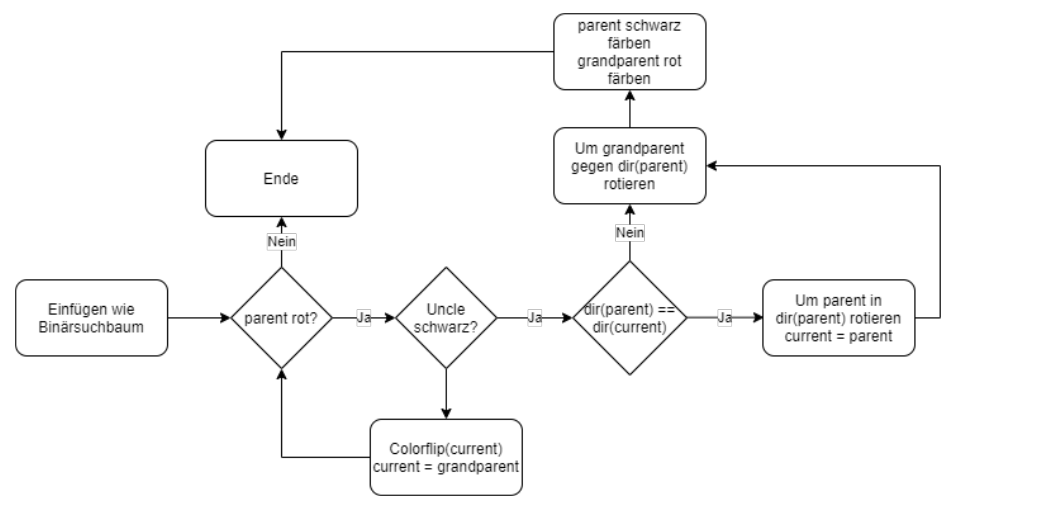
\includegraphics[width=250px]{prog1.png}
  \caption{Programmablaufplan Einfügen}
\end{wrapfigure}

Beim \textbf{Einfügen} ist die erste Neuerung, dass die neuen Knoten immer rot sind. 
Also kann nur Eigenschaft 2 invalidiert werden, nachdem dieser Algorithmus durchgeführt wurde. 
Das passiert genau dann, wenn der Parent des eingefügten Knotens rot war. Man erweitert den Standardalgorithmus nun um eine weitere Funktion, 
die diesen Fall überprüft und dann nach bestimmten Kriterien Rotationen und Colorflips durchführt, bis der Baum wieder ein valider \gls{rbt} ist.

Der Algorithmus wird iterativ auf den Baum solange angewandt, bis der Parent des aktuellen Knotens nicht rot ist. 
Begonnen wird beim neu eingefügten Knoten. Der \textbf{1. Fall} tritt ein, wenn der Uncle des behandelten Knotens rot ist. 
Dann wird einfach ein Colorflip ausgeführt und man setzt den Algorithmus beim Grandparent fort.
Im \textbf{2. Fall} ist der Uncle schwarz und der aktuelle Knoten zeigt in dieselbe Richtung wie der Parent. 
Dann wird eine Rotation ausgeführt in die Richtung, in die der Parent zeigt. Eine Linksrotation wenn er nach links zeigt und ansonsten eine Rechtsrotation.
Das Schöne hier ist nun, dass dieser zweite Fall direkt zum \textbf{3. Fall} führt.
Er kann jedoch auch erreicht werden, wenn der Parent und der aktuelle Knoten in unterschiedliche Richtungen zeigen. Dann wird in die Richtung des Parents um den Grandparent rotiert, der Parent schwarz und der Grandparent rot gefärbt und der Algorithmus wird beendet.
So braucht man maximal 2 Rotationen oder $h/2$ Colorflips ($h$ ist die Länge des längsten Paths von der Root zu einem Leaf oder wird auch Höhe des Baums genannt).

\begin{wrapfigure}{l}{0pt}
  \centering
  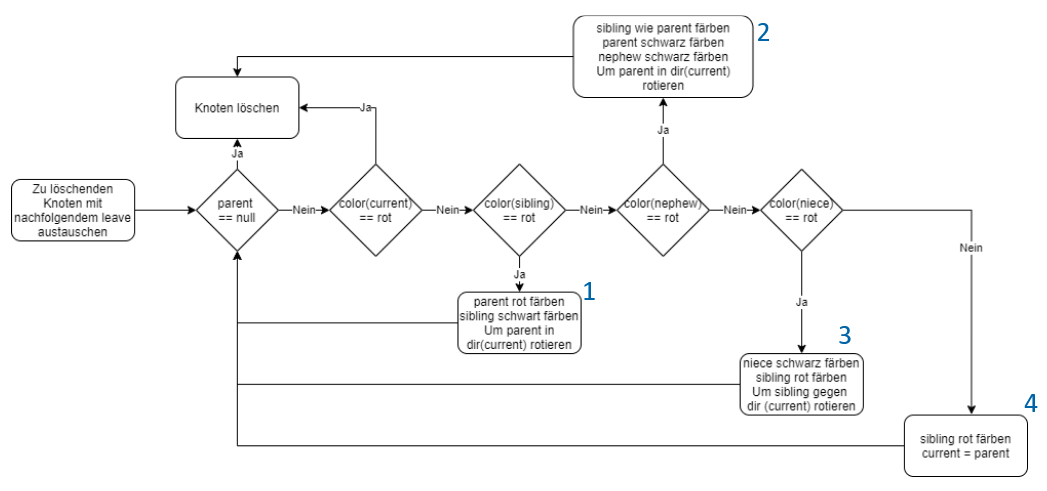
\includegraphics[width=300px]{prog2.png}
  \caption{Programmablaufplan Löschen}
  \label{del-tr}
\end{wrapfigure}

Der letzte Algorithmus, der angepasst werden muss, ist das \textbf{Löschen} von Knoten im Baum. Es muss wieder einen Algorithmus geben, 
der den Baum nach dem Entfernen eines Knotens wieder zu einem validen \gls{rbt} macht. 

Nun kommt es zu einer Verletzung der Regeln, wenn man einen schwarzen Knoten entfernt, weil dann nicht mehr alle Paths dieselbe Anzahl von ihnen haben. 
Der folgende Algorithmus ist wieder als Ablaufplan in Abbildung \ref{del-tr} dargestellt. 
Auch hier gibt es wieder eine Fallunterscheidung. Diesmal jedoch mit 4 Fällen. Diese sind auch in der Abbildung entsprechend markiert.
Als erstes wird einmal überprüft, ob die Root entfernt wird (also, ob der Knoten überhaupt einen Parent hat) oder ob er rot ist. In diesen Fällen ist der Algorithmus sofort fertig und man kann sicher löschen.

Anderfalls muss nun das Rebalancieren beginnen. Wenn der Sibling des aktuellen Knotens rot ist, wird der Parent rot gefärbt, der Sibling schwarz und es wird in Richtung des aktuellen Knotens um den Parent rotiert.
Wenn der Sibling rot ist, werden dann Niece und Nephew überprüft.
Wenn der Nephew rot ist, dann wird der \textbf{2. Fall} behandelt. In diesem Fall wird der Sibling rot eingefärbt, der Parent und Nephew schwarz und es wird in Richtung des aktuellen Knotens um den Parent rotiert.
Das Besondere hier ist, dass nach diesem Fall der Baum balanciert ist und das Entfernen des Knotens durchgeführt werden kann.
Sonst geht es damit weiter, dass die Farbe der Niece überprüft wird. Ist sie rot, dann wird der Algorithmus für den \textbf{3. Fall} ausgeführt. Hier wird die Niece schwarz gefärbt, der Sibling rot und dann um den Sibling in Richtung des aktuellen Knotens rotiert.
Und wenn alle oben genannten Bedingungen nicht zutreffen, sind alle genannten Knoten schwarz und es wird einfach der Sibling rot gefärbt und der Algorithmus beim Parent fortgesetzt. Das ist der \textbf{4. Fall}.
Die 4 Abbildungen unten illustrieren die Unterbäume für die 4 Fälle. Der Knoten, der mit $x$ bezeichnet ist, ist der zu entfernende Knoten. Es ist ein Leaf oder Halfleaf per Definition. 

Als kurze Erklärung, warum die Algorithmen so definiert sind, muss man zuerst das Problem aufzeigen. Im Unterbaum des zu löschenden Knotens fehlt ein schwarzer Knoten. Nun gibt es 2 Ansätze, dieses Problem zu lösen. Entweder man versucht
einen neuen schwarzen Knoten zu erzeugen, damit die Balance wieder hergestellt wird. Das sind die Fälle 1, 2, 3. Allerdings muss dabei sichergestellt werden, dass die anderen Regeln des \gls{rbt} danach weiterhin gelten. Oder man probiert aus dem benachbarten Unterbaum einen schwarzen Knoten zu entfernen (Fall 4).
Hier besteht nun das Problem, dass sich die Anzahl der schwazen Knoten der Pfade, die durch den Parent und dessen Sibling führen, unterscheiden. Also muss man auch einen schwarzen Knoten aus dem Unterbaum des Siblings des Parents entfernen. Und so weiter bis man an der Root ankommt.  
Auch hier kann man zeigen, dass die Anzahl der Ausführungen der einzelnen Algorithmen für die Fälle begrenzt ist, der gesamte Algorithmus also terminiert.

\begin{figure}[h]
  \begin{minipage}[t]{.21\linewidth}
    \centering
    \begin{tikzpicture} [
      inner sep = 0,
      level 1/.style = { sibling distance = 2cm },
      level 2/.style = { sibling distance = 1cm },
      every node/.style={thick, draw, circle, minimum width = 0.5cm}
      ]
    
      \node [black] {p}
      child [-latex] { node[black] {x} } 
      child [-latex] { node [red] {s} child { node[black] {ni} } child { node[black] {ne} } };
    \end{tikzpicture}
    \caption{1. Fall}
  \end{minipage}
  \hfill
  \begin{minipage}[t]{.21\linewidth}
    \centering
    \begin{tikzpicture} [
      inner sep = 0,
      level 1/.style = { sibling distance = 2cm },
      level 2/.style = { sibling distance = 1cm },
      every node/.style={thick, draw, circle, minimum width = 0.5cm}
      ]
    
      \node [black] {p}
      child [-latex] { node[black] {x} } 
      child [-latex] { node [black] {s} child { node[red] {ni} } child { node[red] {ne} } };
    \end{tikzpicture}
    \caption{2. Fall}
  \end{minipage}
  \hfill
  \begin{minipage}[t]{.21\linewidth}
    \centering
    \begin{tikzpicture} [
      inner sep = 0,
      level 1/.style = { sibling distance = 2cm },
      level 2/.style = { sibling distance = 1cm },
      every node/.style={thick, draw, circle, minimum width = 0.5cm}
      ]
    
      \node [black] {p}
      child [-latex] { node[black] {x} } 
      child [-latex] { node [black] {s} child { node[black] {ni} } child { node[red] {ne} } };
    \end{tikzpicture}
    \caption{3. Fall}
  \end{minipage}
  \hfill
  \begin{minipage}[t]{.21\linewidth}
    \centering
    \begin{tikzpicture} [
      inner sep = 0,
      level 1/.style = { sibling distance = 2cm },
      level 2/.style = { sibling distance = 1cm },
      every node/.style={thick, draw, circle, minimum width = 0.5cm}
      ]
    
      \node [black] {p}
      child [-latex] { node[black] {x} } 
      child [-latex] { node [black] {s} child { node[black] {ni} } child { node[black] {ne} } };
    \end{tikzpicture}
    \caption{4. Fall}
  \end{minipage}
  \hfill

\end{figure}
\cite{YTDelete}

\pagebreak
\section{Implementierung} \label{impl}
Wie schon in den vorhergenden Kapiteln beschrieben, handelt es sich bei den Bäumen um eine Datenstruktur, in die der Nutzer beliebig Daten mit einem bestimmten Schlüssel einfügen kann.

Die Implementierung stellt deswegen 3 Funktionen bereit, mit denen man nach einem bestimmten Schlüssel im Baum suchen kann, man einen neuen Schlüssel zusammen mit einem Datensatz einfügen kann und einen Schlüssel und den Datensatz wieder aus dem Baum löschen kann.

\subsection{Generics in C}
Bei der Implementierung in \cpl gab es dabei einige Schwierigkeiten, die man lösen musste. Es beginnt damit, dass \cpl keine objekt-orientierte Programmiersprache ist und keine eingebaute Möglichkeit für \glspl{gns} hat.
Nun kann man dieses Problem auf verschiedene Weisen lösen. Den Wert, der bei jedem Knoten des Baums gespeichert werden soll, lässt sich ganz simple als Void-Pointer (\lstin{void*}) implementieren, sodass man die Daten beispielsweise auf dem \gls{hp} ablegen kann
und mithilfe eines Casts den Pointer der Daten (z.B. \lstin{int*}) zu \lstin{void*} umwandeln kann. Das erlaubt es, beliebige Datentypen und sogar Structs in den Baum einzufügen.
Diese Variante ist möglich, da die Nutzerdaten auf die Suche nach einem Knoten keinen Einfluss haben.

Anders ist es bei der Implementierung der Schlüssel. Hier muss sichergestellt sein, dass diese untereinander vergleichbar sind, sodass man die Suche, wie im Kapitel \ref{def} beschrieben, durchführen kann.
Man könnte Gebrauch von \glspl{uns} in \cpl machen, in denen man die numerischen Datentypen als mögliche Schlüssel anbietet.

\begin{lstlisting}[language=C]
union RBTreeKey {
  char c;
  short s;
  int i;
  long long l;
  float f;
  double d;
}
\end{lstlisting}

Zusätzlich müsste man dazu noch angeben, welchen Datentyp man in seinem Code nutzt (z.B. mithilfe einer \gls{mc}). Dieser Ansatz ist allerdings sehr unflexibel, weil man auf die Datentypen, die im \lstin{union RBTreeKey} vom Programmierer festgelegt sind, beschränkt ist.

Ein bessere Ansatz ist es, eine \gls{mc} zu definieren, die den Typen der Schlüssel enthält. Zusätzlich kann man noch eine 2. und 3. \gls{mc} erstellen, die die Kleiner-Als- und Ist-Gleich-Operatoren definieren.
Das ermöglicht es, beliebige Datentypen als Schlüssel zu verwenden (sogar Structs), solange man die Vergleichsmacros richtig in der \gls{mc} angeben kann.

\begin{lstlisting}[language=C]
#define T int
#define TEQUAL(x, y) ((x) == (y))
#define TLESS(x, y) ((x) < (y))
\end{lstlisting}

Genau diese Implementierung wurde auch gewählt. Im Usercode müssen nur der Typ \lstin{T} und die Vergleichsoperationen \lstin{TLESS} und \lstin{TEQUAL} definiert werden. Einziger Nachteil ist, dass man im selbe \gls{sc} nicht meherere verschiedene Varianten von Schlüsseldatentypen nutzen kann.

\subsection{Knoten als Struct}
Wie schon in Kapitel \ref{def} beschrieben, sind Bäume nichts anderes als ein 3-Tupel $(l, k, r)$.
$l$ und $r$ sind die Unterbäume und $k$ ist die Root des Baumes.
Jeder Knoten enthält somit seinen Schlüssel und eine Referenz auf den linken und rechten Unterbaum.
In \cpl wird der Baum nun als verkettete Liste von Knoten dargestellt.
Im \lstin{struct Node} wird der generische Schlüssel \lstin{T *key} und zugehörige Wert \lstin{void *value} gespeichert.
Zusätzlich gibt es jeweils einen Pointer zum linken und rechten Child, welche die Roots der entsprechenden Unterbäume sind. Zusätzlich wird auch noch ein Pointer auf den Parent gespeichert,
da man diesen ziemlich oft in den Algorithmen zum Einfügen und Löschen von Knoten benötigt und man so den Quellcode etwas vereinfachen kann.

Natürlich gibt es im Knoten auch noch ein Feld, welches die Farbe speichert. Diese ist später wichtig, weil sie zum Balancieren des Baumes benötigt wird.
Dieses findet während des Einfügens und Löschens neuer Knoten in den Baum statt. Die Werte, die die Farbe annehmen kann, werden durch die \glspl{mc} \lstin{RB_TREE_RED} und \lstin{RB_TREE_BLACK} definiert.

Zusätzlich existiert ein weiterer Struct für den Baum selbst, welcher allerdings nur als Handle für die Funktionen dient. Er speichert die Root
und die Anzahl der eingefügten Knoten. Diese wird benötigt, damit man die Worst-Case-Höhe des Baums berechnen kann
\footnote{Die Worst-Case-Höhe wird für eine kleine Optimierung benötigt. Im Kapitel \ref{tr} wird beschrieben, wie man die Bäume traversiert.
Das ist normalerweise eine rekursive Operation, die ich jedoch iterativ implementiert habe. Dafür werden \glspl{st} benötigt, die sich dynamisch vergrößern, falls sie überlaufen würden.
Ich habe diese Stacks jedoch so implementiert, dass man sie mit einer initialen Größe erstellen kann. Die Worst-Case-Höhe des Baums gibt nun ungefähr die größte \gls{rcd} an, welche bei mir der größten Anzahl an Elementen auf dem Stack entspricht.
Somit kann ich dem Stack von Anfang an schon genug Platz geben, sodass er sich nicht so oft vergrößern muss, was mit einem Aufruf von \lstin{reallocarray()} verbunden.
Dabei wird ein großer Speicherbereich kopiert, was das Programm unnötig verlangsamt, wenn man zu oft mehr Speicher im Stack benötigt.
}.

\begin{lstlisting}[language=C]
#define RB_TREE_RED     1U
#define RB_TREE_BLACK   0U

struct Node;

struct Node {
    void *value;

    T *key;

    struct Node *left;
    struct Node *right;
    struct Node *parent;

    uint8_t color;
};

struct RBTree {
    struct Node *root;

    size_t node_count;
};
\end{lstlisting}

Zusätzlich existieren 2 Helfer-Funktionen, die jeweils eine Instanz von diesem Struct für den Nutzer erstellen und auch wieder freigeben. Der Baum wird durch die \lstin{create_tree} Funktion auf dem Heap abgespeichert und es wird lediglich ein Pointer zu ihm ausgegeben.
Das Löschen des Baumes wird durch \lstin{free_tree} implementiert. Dieses ist auf keinen Fall trivial, weil es Bottom-Up durchgeführt werden muss und somit nicht durch den Nutzer selbst implementiert werden sollte.

Die Signatur dieser Funktionen sieht man im unteren Listing.

\begin{lstlisting}[language=C]
struct RBTree* create_tree();
void free_tree(struct RBTree *rbtree);
\end{lstlisting}

\subsection{Suche nach Knoten} \label{sea}
Eine der wichtigsten Operation, auf die auch später das Einfügen und das Löschen von Knoten aufbaut, ist die Suche im Baum. Diese ist normalerweise als rekursiver Algorithmus definiert, lässt sich aber auch ziemlich einfach iterativ implementieren.
Grundsätzlich wurde im Code dieser Arbeit auf \gls{rec} verzichtet und entweder ein iterativer Ansatz verwendet oder ein selbst implementierter \gls{st}, um \glspl{sof} zu vermeiden.

Die Funktion, die die Suche implementiert, akzeptiert einen Pointer zum Baum, den zu suchenden Schlüssel und einen Pointer, in den der Pointer des gefundenen Knotens geschrieben werden kann, wenn vorhanden.

\begin{lstlisting}[language=C]
uint8_t search_node(struct RBTree* rbtree, T* key, struct Node** node);
\end{lstlisting}

Der Algorithmus selbst speichert den aktuellen Knoten in der Variable \lstin{struct Node* current}. Diese wird mit der Root initialisiert. Anschließend wird iterativ entweder der linke oder der rechte Unterbaum besucht, abhängig davon, ob der Schlüssel, nachdem gesucht wird, kleiner oder größer als der Schlüssel des aktuellen Knotens ist.
Wenn er kleiner ist, wird der linke Unterbaum besucht, sonst der Rechte. Dies geschieht, in dem \lstin{current} entweder das linke oder rechte Child des aktuellen Knotens zugewiesen wird.

Die \lstin{while}-Schleife bricht ab, wenn der Schlüssel gefunden wurde oder das nächste Child \lstin{NULL} ist. Im letzteren Fall wird ein Fehlercode returned und dem Ausgabe Pointer \lstin{NULL} zugewiesen, weil der Schlüssel nicht im Baum vorhanden ist.
Ansonsten kann man der Ausgabe einfach \lstin{current} zuweisen und den Erfolgswert returnen, der anzeigt, dass es keinen Fehler gab (mehr dazu in Kapitel \ref{err}).

\begin{lstlisting}[language=C]
struct Node *current  = rbtree->root;

while (current != NULL) {
    if (TEQUAL(*(current->key), *(key))) break;
    current = (TLESS(*key, *(current->key))) ? current->left : current->right;
}

if (current == NULL) {
    *node = NULL;
    return RB_TREE_KEY_ERROR;
}

*node = current;
return RB_TREE_SUCCESS;
\end{lstlisting}

\subsection{Einfügen von Knoten}

\subsubsection{Einfügen des neuen Knotens}
Eine weitere wichtige Operation ist das Einfügen von Daten in den Baum. Dabei müssen die zwei Eigenschaften der Datenstruktur erhalten bleiben. Diese sind die sortierte Reihenfolge und, dass der Baum ein valider \gls{rbt} ist.
Das Listing unten zeigt die Signatur der Funktion, die das Einfügen durchführt. Sie akzeptiert einen Pointer zu dem Baumstruct \lstin{struct RBTree* rbtree}, einen Pointer zum Schlüssel des neuen Knotens \lstin{T* key} und optional Daten, die auch im Knoten gespeichert werden sollen \lstin{void* value} (dieser Wert kann auch \lstin{NULL} sein).

\begin{lstlisting}[language=C]
uint8_t insert_node(struct RBTree* rbtree, T* key, void* value);
\end{lstlisting}

Die Implementierung sorgt zuerst dafür, dass der neue Knoten an die richtige Stelle im Baum eingefügt wird und stellt danach (wenn nötig) sicher, dass es immer noch ein valider \gls{rbt} ist.

Das Einfügen des Knotens in den Baum kann nun analog zur Suche implementiert werden.
Der Unterschied liegt darin, dass man den Baum durchsucht, bis man bei \lstin{NULL} ankommt.
Beim Suchen war der Fehlerfall, dass es keinen Knoten mit dem zu suchenden Schlüssel gab, aber während des Einfügens ist das die Annahme, die getroffen wird.
Der Schlüssel, den der Nutzer neu hinzufügen will, sollte noch nicht im Baum enthalten sein. Damit ist der erreichte \lstin{NULL}-Pointer nach der Logik des Baums genau die Stelle, an der der neue Knoten mit dem neuen Schlüssel eingefügt werden muss.

Der Grund, warum hier der Pointer zum Vorgänger-Knoten \lstin{previous} zusätzlich gespeichert werden muss ist,
dass \lstin{NULL} nicht auf eine valide Structinstanz zeigt, sondern lediglich anzeigt, dass es keinen Knoten an dieser Stelle gibt.
Somit kann man auch nicht den Parent von \lstin{NULL} abfragen und man muss diese Information in einer zustätzlichen Variablen zwischenspeichern.

\begin{lstlisting}[language=C]
struct Node *previous = NULL;
struct Node *current  = rbtree->root;

while (current != NULL) {
    previous = current;
    current  = (TLESS(*key, *(previous->key))) ? previous->left : previous->right;
}
\end{lstlisting}

Nun wird eine neue Instanz von \lstin{struct Node} erstellt. Das erledigt die Helfer-Funktion \lstin{_create_node}, welche den neuen Knoten auf dem Heap abspeichert und den Pointer auf ihn ausgibt.
In ihr wird auch direkt sichergestellt, dass der neu allozierte \gls{hp}-Speicher korrekt initialisiert und die Farbe auf rot gesetzt wird.
Der neue Knoten muss dann an den Parent vom erreichten \lstin{NULL}-Pointer entweder links oder rechts angehangen werden.

\begin{lstlisting}[language=C]
struct Node *new_node = _create_node(key, value);
if (TLESS(*key, *(previous->key))) {
    previous->left = new_node;
} else {
    previous->right = new_node;
}
new_node->parent = previous;
\end{lstlisting}

Es gibt auch noch den Spezialfall, dass ein Knoten in einen noch leeren \gls{rbt} eingefügt werden soll.
Hier muss dann der Pointer auf die Root im \lstin{struct RBTree} gesetzt werden. Deswegen wird, bevor der oben angebene Algorithmus ausgeführt wird noch überprüft,
ob der Nutzer den leeren Baum als Eingabe in die Funktion gegeben hat.
Das Gute ist, dass man in diesem Fall auch gar nicht den Baum durchsuchen muss, sondern sofort weiß, dass der neue Knoten die Root selbst ist.
Es darf allerdings nicht vergessen werden, dass durch \lstin{_create_node} die Farbe des neuen Knotens auf rot gesetzt wurde. Sie muss deswegen noch zu schwarz geändert werden,
weil die Root des \gls{rbt} immer schwarz sein muss.
\begin{lstlisting}[language=C]
if (rbtree->root == NULL) {
  rbtree->root = new_node;
  rbtree->root->color = RB_TREE_BLACK;
}
\end{lstlisting}

\subsubsection{Balancieren des Baums (Einfügen)}
Nach dem Einfügen in den Baum kann es dazu kommen, dass die Regeln des \glspl{rbt} verletzt werden.
Dieser Fall tritt dann ein, wenn der Parent des neuen Knotens rot ist, denn dann sind 2 aufeinanderfolgende rote Knoten im Baum, was nicht sein darf (siehe \ref{def}).

Wenn der obige Fall eintritt, muss einer der in Kapitel \ref{def} beschriebenen Algorithmen ausgeführt werden, damit der Baum wieder alle Eigenschaften erfüllt und ein valider \gls{rbt} wird.
Das hat den Nebeneffekt, dass der Baum dabei besser im Durchschnitt ausbalanciert wird.
In der Implementierung wurden Helferfunktionen implementiert, die den Colorflip und die Rotationen am Baum durchführen.

Das untere Listing zeigt einen Auszug aus der Funktion, welche die Baumrotation durchführt (nur die Linksrotation).

\begin{lstlisting}[language=C]
struct Node *child = start_node->right;
if (start_node == rbtree->root) rbtree->root = child;
child->parent = start_node->parent;

if (start_node->parent != NULL) {
  if (start_node->parent->left == start_node) start_node->parent->left = child;
  else start_node->parent->right = child;
}

start_node->right = child->left;
if (start_node->right) start_node->right->parent = start_node;

child->left = start_node;
start_node->parent = child;
\end{lstlisting}

Hier zeigt sich der Vorteil der Implementierung als Verkettung von Pointern. Die Rotation kann einfach durch das Austauschen von Child- und Parent-Pointern implementiert werden.

Die Funktion, die den Colorflip implementiert, wird hier nicht genauer betrachtet, weil sie tatsächlich nur das \lstin{color} Feld im Struct ändert.

Nachdem die Helferfunktionen besprochen wurden, kann nun endlich mit dem Rebalancieren begonnen werden.
Die Funktion, die diesen entsprechenden Algorithmus dafür implementiert, heißt \lstin{fix_tree_insert}. Ihre Signatur befindet sich im unteren Listing.

\begin{lstlisting}[language=C]
void fix_tree_insert(struct Node *start_node, struct RBTree *rbtree)
\end{lstlisting}

\lstin{start_node} ist dabei der Knoten, der die Eigenschaften eines \gls{rbt} verletzt, also der Knoten, der zuletzt eingefügt wurde.

Unten kann man nun die Implementierung der Funktion sehen.
Als erstes werden 2 Pointer angelegt, die den aktuell betrachteten Knoten und seinen Parent speichern.
Das ist wichtig, weil es passieren kann, dass der Algorithmus mehrere Schritte benötigt.
Das ist auch der Grund, warum sich alles innerhalb einer \lstin{while}-Schleife befindet, nämlich damit solange rebalanciert wird,
bis die Abbruchbedingung erreicht wird (siehe Kapitel \ref{def}).

Wie schon in Kapitel \ref{def} beschrieben, gibt es verschiedene Fälle, die betrachtet werden müssen.
Je nach Farbe des Uncle-Knotens und Richtung des Parents werden Colorflips und Rotationen durchgeführt.
Dafür können hier nun die Helferfunktionen, die in den letzten Abschnitten beschrieben wurden, genutzt werden.
Der Vorteil daran ist, dass diese auch gleich noch bestimmte Fehlerfälle abfangen, sodass man sich viel Codeduplizierung ersparen kann.

Als letztes wird noch die Farbe der Root auf \lstin{RB_TREE_BLACK} gesetzt, weil es vorkommen kann,
dass sie am Ende rot ist. Die Eigenschaften von \gls{rbt} schreiben jedoch vor, dass die Root immer schwarz sein muss.
Hier wurde bewusst auf eine \lstin{if}-Abfrage verzichtet, um Instruktionen zu sparen.

\begin{lstlisting}[language=C]
struct Node *current = start_node;
struct Node *parent = start_node->parent;

while (parent != NULL && parent->color == RB_TREE_RED && current->color == RB_TREE_RED) {
    if (parent->parent == NULL) break;

    struct Node *uncle = get_uncle(current);

    if (get_color(uncle) == RB_TREE_BLACK) {
        if (get_direction(parent) != get_direction(current)) {
            rotate(parent, get_direction(parent), rbtree);
            current = parent;
            parent = current->parent;
        } else {
            struct Node *grandparent = get_grandparent(current);
            rotate(grandparent, !get_direction(parent), rbtree);
            parent->color = RB_TREE_BLACK;
            grandparent->color = RB_TREE_RED;
            break;
        }
    } else if (get_color(uncle) == RB_TREE_RED) {
        color_flip(current);
        if (parent->parent == NULL) break;

        struct Node *uncle = get_uncle(current);
        current = get_grandparent(current);
        parent = current->parent;
    }
}

rbtree->root->color = RB_TREE_BLACK;

\end{lstlisting}

\subsection{Löschen von Knoten}

Die letzte Operation, die die Daten im Baum verändert, ist das Löschen von Knoten.
Sie ist wohl auch der komplizierteste Algorithmus, weil sie sehr viele Fälle betrachtet
und viele Grenzfälle abfangen muss.

In meiner Implementierung findet das Löschen in 3 Schritten statt. Als erstes wird der Knoten, der gelöscht werden soll,
mit einem Leaf des Baumes ausgetauscht, falls er noch keines ist. Danach kann dieser sicher entfernt werden, ohne dass der Baum
in mehrere Bäume zerfällt. Anschließend wird wieder die Balancierung durchgeführt.
Alle diese Algorithmen wurden wieder in separate Funktionen extrahiert.

Die Funktion, die der Nutzer meiner Datenstruktur aufruft, um einen Knoten zu entfernen, heißt \lstin{delete_node}.
Sie hat folgende Signatur:

\begin{lstlisting}
uint8_t delete_node(struct RBTree* rbtree, T* key);
\end{lstlisting}

\lstin{T* key} ist hier der Schlüssel des Knotens, der gelöscht werden soll.

Es wird damit begonnen, dass der Knoten mit dem entsprechenden Schlüssel \lstin{key} gesucht wird.
Dafür kann die \lstin{search}-Funktion verwendet werden, die im Kapitel \ref{sea} etabliert wurde.

\begin{lstlisting}[language=C]
struct Node *node_to_delete = NULL;
search_node(rbtree, key, &node_to_delete);
\end{lstlisting}

Als nächstes wird dann der Algorithmus durchgeführt, der den zu löschenden Knoten mit einem Blatt austauscht.
Das Blatt, mit dem getauscht wird, ist so zu wählen, dass nach der Löschung die Inorder-Traversierungsreihenfolge korrekt ist.
Das alles wird durch die Funktion \lstin{swap_to_leaf} implementiert. Sie gibt dann den Pointer zum Blatt aus \lstin{x}, welches entfernt werden kann.
\begin{lstlisting}[language=C]
struct Node *x = swap_to_leaf(node_to_delete);
\end{lstlisting}

Dann wird noch die \lstin{fix_tree_delete}-Funktion aufgerufen.
Sie ist das Äquivalent zu \lstin{fix_tree_insert}, welches nach dem Einfügen den Baum balanciert,
aber etwas komplizierter in ihrer Implementierung.

\begin{lstlisting}
fix_tree_delete(x, rbtree);
\end{lstlisting}

Jetzt wird noch überprüft, ob die Root gelöscht werden soll, was bedeutet,
dass sie der einzige Knoten im Baum ist. Hier müssen dann einige Felder im \lstin{rbtree}-Struct
verändert werden. Es werden dann alle Pointer, die auf den Knoten zeigen, zu \lstin{NULL} geändert,
was ihn effektiv aus dem Baum entfernt. Danach wird der zu löschende Knoten freigegeben.

\begin{lstlisting}[language=C]
if (rbtree->root == x) {
    _free_node(rbtree->root);
    rbtree->root = NULL;
    return RB_TREE_SUCCESS;
}

if (get_direction(x) == RB_TREE_LEFT_CHILD) x->parent->left = NULL;
else x->parent->right = NULL;

_free_node(x);
\end{lstlisting}

Es wurden in diesem einführenden Abschnitt einige Funktionen genannt, die noch als Blackbox
betrachtet wurden. Auf deren Funktionsweise wird in den nächsten Kapiteln näher eingegangen.

\subsubsection{Austauschen mit Blatt}

Das Austauschen findet in der Funktion \lstin{swap_to_leaf} statt, deren Signatur sich im unteren Listing befindet.

\begin{lstlisting}
struct Node* swap_to_leaf(struct Node *node_to_delete);
\end{lstlisting}

\lstin{node_to_delete} ist der Pointer zum Knoten, der mit einem Leaf getauscht werden soll. Das darf aber nicht irgendein Leaf sein, sondern das, welches den nächstkleineren bzw -größeren Schlüssel hat, damit
nach dem Entfernen von \lstin{node_to_delete} die Inorder-Reihenfolge erhalten bleibt.

In der Funktion selbst muss nun der Knoten mit der oben genannten Eigenschaft gefunden werden. Dies geschiet, in dem man erst im linken Unterbaum von \lstin{node_to_delete} des Child sucht, welches sich am weitesten rechts befindet.
Und falls es das nicht gibt, sucht man im rechten Unterbaum nach dem Knoten, der sich am weitesten links befindet. Das sind die Knoten, die in der Inorder-Reihenfolge direkt vor bzw. nach dem zu löschenden Knoten kommen.
Das wird durch die Helfer-Funktionen \lstin{get_next_smallest} bzw. \lstin{get_next_largest} implementiert. Im unteren Listing kann man beispielhaft die Implementierung einer dieser Funktionen sehen:

\begin{lstlisting}[language=C]
void get_next_largest(struct Node *start, struct Node **next_largest)
{
    struct Node *current  = start;
    while (current->left != NULL) current = current->left;
    *next_largest = current;
}
\end{lstlisting}

Wenn keiner der beiden oberen Fälle eintritt, dann ist \lstin{note_to_delete} bereits ein Leaf und der Algorithmus gibt den Knoten selbst aus.

Ansonsten werden mithilfe der Funktion \lstin{swap} die Schlüssel und Daten des Leafs und von \lstin{note_to_delete} einfach ausgetauscht und es wird der Pointer zum Leaf ausgegeben.
Unten kann man die Implementierung für den Fall des linken Unterbaums sehen. 
Die für den rechten Unterbaum kann man im Code nachschlagen.

\begin{lstlisting}[language=C]
struct Node *next_smallest =  NULL;
get_next_smallest(node_to_delete->left, &next_smallest);
leaf = next_smallest;
swap((void**)&node_to_delete->key, (void**)&next_smallest->key);
swap(&node_to_delete->value, &next_smallest->value);
\end{lstlisting}

\subsubsection{Balancieren des Baumes (Löschen)}
Ähnlich wie beim Einfügen in den Baum, muss auch nach dem Entfernen aus dem Baum rebalanciert werden.
Die Signatur der Funktion, die den entsprechenden Algorithmus implementiert, ist so definiert:
\begin{lstlisting}
void fix_tree_delete(struct Node *x, struct RBTree *rbtree);
\end{lstlisting}

\lstin{x} ist hier der Pointer auf den Knoten, der aus dem Baum gelöscht werden soll. Man kann hier annehmen, dass er ein Leaf oder Halfleaf ist,
denn die \lstin{swap_to_leaf}-Funktion wird vorher auf \lstin{node_to_delete} angewandt, sodass immer nur Leaves oder Halfleaves gelöscht werden müssen.

Ähnlich wie beim Einfügen gibt es auch hier wieder Fälle, die der Code abarbeiten muss, abhängig von der Farbe bestimmter Knoten.
Der Algorithmus befindet sich in einer \lstin{while}-Schleife, weil es auch hier wieder passieren kann, dass es mehrere Durchläufe gibt, bevor der Baum balanciert ist.

Die ersten beiden Bediengungen \lstin{x->parent == NULL} und \lstin{get_color(x) == RB_TREE_RED} terminieren den Algorithmus sofort.
Die erste Bediengung trifft genau dann zu, wenn die Root entfernt wird. Danach entsteht allerdings der leere Baum, der nach Definition balanciert ist, also muss man hier nichts mehr tun.
Da die Eigenschaften von \gls{rbt} beim Löschen nur dann verletzt werden, wenn man einen schwarzen Knoten entfernt,
kann man auch sofort abbrechen, wenn die Farbe von \lstin{x} rot ist, was der zweiten Bediengung entspricht.

Alle anderen Zweige des \lstin{if}-Konstrukts entsprechen nun den 4 Fällen.
Wie diese sich genau aufbauen, und warum sie so definiert sind, wurde bereits in Kapitel \ref{def} beschrieben. Deswegen wird dieser Teil hier nicht noch einmal im Detail erklärt.

Was es noch anzumerken gibt ist, dass der Fall 2 ebenfalls zum Terminieren des Algorithmus führt, weswegen sich dort ein \lstin{break} am Ende des Codeblocks befindet.
Es ist durch die Definition des Algorithmus sichergestellt, dass dieser immer terminiert, also irgendwann die Root erreicht oder den Fall 2 (siehe Kapitel \ref{def}).

Das untere Listing zeigt die gesamte Implementierung der Funktion.

\begin{lstlisting}[language=C]
while(1) {
    if (x->parent == NULL) {
        break;
    } else if (get_color(x) == RB_TREE_RED) { break; } 
      else if (get_color(get_sibling(x)) == RB_TREE_RED) {
        x->parent->color = RB_TREE_RED;
        get_sibling(x)->color = RB_TREE_BLACK;
        rotate(x->parent, get_direction(x), rbtree);
    } else if (get_color(get_nephew(x)) == RB_TREE_RED) {
        get_sibling(x)->color = x->parent->color;
        x->parent->color = RB_TREE_BLACK;
        get_nephew(x)->color = RB_TREE_BLACK;
        rotate(x->parent, get_direction(x), rbtree);
        break;
    } else if (get_color(get_niece(x)) == RB_TREE_RED) {
        get_niece(x)->color = RB_TREE_BLACK;
        get_sibling(x)->color = RB_TREE_RED;
        rotate(get_sibling(x), !get_direction(x), rbtree);
    } else {
        get_sibling(x)->color = RB_TREE_RED;
        x = x->parent;
    }
}
x->color = RB_TREE_BLACK;
\end{lstlisting}
\cite{YTDelete}

\subsection{Generische Baumtraversierung} \label{tr}
Wie schon in der Einleitung erwähnt, bieten \glspl{bt} die Möglichkeit, Daten geordnet zu speichern. Nun benötigt man auch Möglichkeiten, auf die Daten in einer bestimmten Reihenfolge zuzugreifen. Grundsätzlich gibt es 3 Optionen, die man als \gls{tv} bezeichnet, nämlich Inorder-, Preorder- und Postorder-Traversierung.
Alle diese Algorithmen sind rekursiv definiert. \cite[S. 44ff]{aic}  Der untere \gls{psc} stellt dar, wie sie funktionieren.

\begin{algorithm}
  \caption{Traversierungs-Algorithmen}
  \begin{algorithmic}[1]
  \Procedure{Preorder}{nodeptr, VISIT}
    \If {noteptr == NULL}
      \Return
    \EndIf
    \State VISIT(noteptr)
    \State PREORDER(noteptr$\rightarrow$left)
    \State PREORDER(noteptr$\rightarrow$right)
  \EndProcedure
  \Procedure{Inorder}{nodeptr, VISIT}
    \If {noteptr == NULL}
      \Return
    \EndIf
    \State INORDER(noteptr$\rightarrow$left)
    \State VISIT(noteptr)
    \State INORDER(noteptr$\rightarrow$right)
  \EndProcedure
  \Procedure{Postorder}{nodeptr, VISIT}
    \If {noteptr == NULL}
      \Return
    \EndIf
    \State POSTORDER(noteptr$\rightarrow$left)
    \State POSTORDER(noteptr$\rightarrow$right)
    \State VISIT(noteptr)
  \EndProcedure
  \end{algorithmic}
\end{algorithm}
\cite[S. 318ff]{aop}

Dabei ist \lstin{noteptr} der Pointer der Root des Unterbaums (der ganze Baum ist auch ein Unterbaum von sich selbst). Und \lstin{VISIT} stellt dabei einen Funktionspointer dar, der einen \lstin{noteptr} als Parameter akzeptiert und ebenfalls als Argument in die Traversierungsfunktionen gegeben wird.
So ist es dem Nutzer möglich, eine bestimmte Funktion auf alle Knoten anzuwenden.

\begin{lstlisting}[language=C]
uint8_t inorder_traversel(struct RBTree *rbtree, void (*visit)(struct Node*))
{
    struct Node *current = rbtree->root;
    struct Stack *stack = create_stack(_calc_worst_case_height(rbtree));

    while (current != NULL || !is_stack_empty(stack)) {
        if (current != NULL) {
            push(stack, current);
            current = current->left;
        } else {
            struct Node *stack_node;
            pop(stack, &stack_node);
            visit(stack_node);
            current = stack_node->right;
        }
    }
    free_stack(stack);
    return RB_TREE_SUCCESS;
}
\end{lstlisting}

Im oberen Listing kann man am Beispiel der Inorder-Traversierung erkennen, wie die Algorithmen iterativ implementiert wurden. Anstatt den Hardware-\gls{st} zu verwenden, wurde ein Software-\gls{st} \lstin{struct Stack *stack} implementiert.
In diesen werden jeweils die noch zu besuchenden Unterbäume gepushed, und wenn der aktuelle Knoten \lstin{current} \lstin{NULL} ist, wird ein neuer Knoten aus dem \gls{st} geholt.
Dieses Vorgehen simuliert das Verhalten einer rekursiven Funktion, jedoch besteht bei sehr großer \gls{rcd} nicht die Möglichkeit eines \gls{sof}. Die anderen Traversierungsarten wurden auf dieselbe Weise implementiert.

Es kommt auf die genutzte Traversierungsart an, in welcher Reihenfolge man die Knoten besucht. Wenn man Inorder nutzt, dann bekommt man sie nach Schlüsseln aufsteigend sortiert. Das kann man z.B. dafür nutzen, die Schlüssel in geordneter Reihenfolge auszugeben.
Bei der Postorder-Traversierung wird die Root des Unterbaums als letztes besucht. So kann man Bottom-Up-Algorithmen implementieren, die bei den Leaves beginnen und die Root des Baums als letztes behandeln.

Ein sehr praktischen Bespiel dafür ist das Freigeben der \glspl{rbt}. Dabei müssen zuerst die Unterbäume aus dem \gls{hp} gelöscht werden und danach die Root, weil man sonst die Unterbäume zwischenspeichern müsste, da die Pointer zu ihnen in der Root gespeichert sind.
Wenn man diese aber nun als erstes freigibt, würde man keinen Zugriff mehr auf ihre Unterbäume haben.

\begin{lstlisting}[language=C]
void _free_node(struct Node *node)
{
    if (node->key != NULL) free(node->key);
    if (node->value != NULL) free(node->value);
    free(node);
}

void free_tree(struct RBTree *rbtree)
{
    postorder_traversel(rbtree, &_free_node);
    free(rbtree);
}
\end{lstlisting}

Hier wurde die \lstin{VISIT}-Funktion als \lstin{_free_node} implementiert, welche den Schlüssel und den Wert des besuchten Knotens freigibt und dann den Knotenstruct selbst.

\subsection{Fehlerbehandlung} \label{err}
Wie man in vielen vorhergenden Listings bereits sehen konnte, haben die meisten Funktionen als Ausgabetypen \lstin{uint8_t}. (Die Fehlerbehandlung wurde aus den Listings jedoch meistens weggelassen, damit sie nicht zu lang werden.)
Das liegt daran, dass die Funktionen über den Ausgabewert Fehler an den Nutzer zurückgeben. Diese Fehler wurden als \gls{mc} definiert und durch sie können verschiedene Fehlerarten unterschieden werden.

\begin{lstlisting}[language=C]
#define RB_TREE_SUCCESS             0U
#define RB_TREE_OUT_OF_MEM          1U
#define RB_TREE_KEY_ERROR           2U
#define RB_TREE_NULL_ERROR          3U
#define RB_TREE_DUPLICATE_KEY_ERROR 4U
\end{lstlisting}

In meiner Implementierung repräsentiert die 0 immer, dass es keinen Fehler gab.
\lstin{RB_TREE_OUT_OF_MEM} wird von Funktionen verwendet, die dynamisch Speicher allozieren und das Betriebssystem nicht mehr genug zur Verfügung stellt.
Die einzige Funktion, die den Fehler nutzt, ist \lstin{insert_node}, nämlich genau dann, wenn kein neuer Knoten erstellt werden kann.
Hierbei wird der Fehler allerdings nicht ausgegeben, sondern das Programm wird mit \lstin{exit(RB_TREE_OUT_OF_MEM)} beendet.
Ein \lstin{RB_TREE_KEY_ERROR} wird von \lstin{search_node} ausgegeben, wenn der zu suchende Schlüssel im Baum nicht existiert.
Funktionen, die Pointer als Argumente akzeptieren, geben einen \lstin{RB_TREE_NULL_ERROR} Fehler aus, wenn mindestens einer dieser Pointer \lstin{NULL} ist.
Und ein \lstin{RB_TREE_DUPLICATE_KEY_ERROR} wird ausgegeben, wenn man \lstin{insert_node} einen Schlüssel übergibt, der bereits im Baum existiert und man doppelte Schlüssel und implizites Überschreiben mithilfe der \lstin{RB_TREE_DUPLICATE_KEYS} \gls{mc} deaktiviert hat.

\section{Implementierungsvarianten}

\subsection{Rekursive Implementierung} 
Wie schon häufig im Kapitel \ref{impl} erwähnt, kann man auch die Suche und die Traversierung direkt als rekursive Funktionen, die sich selbst aufrufen, implementieren. Das wurde auch durchgeführt. Im Kaptiel \ref{ben2} kann man die Unterschiede bezüglich der Laufzeit der Programme sehen.
Interssierte Leser können sich den Quelltext in der Datei \lstin{rbtree_h.c} ansehen. Auf eine genauere Diskussion der Implementierung wird hier verichtet.

\subsection{Kekule Zahlen}
Theoretisch gibt es auch eine Möglichkeit die Baumstruktur als \gls{arr} von Knoten darzustellen und bessere Cacheladezeiten zu bekommen.
Das größte Problem bei der Implementierung als verkettete Datenstruktur ist, dass die einzelnen Knoten stark verstreut im Heap abgespeichert sind und somit es zu vielen Cache Misses kommt. Diese Streuung kommt durch die Implementierung von \lstin{malloc} in der \cpl-Standart-Bibliothek zustande ("The order and contiguity of storage allocated by successive calls to malloc() is unspecified." \cite{IEEEmalloc}). Das verlangsamt das Programm.

Kekule-Zahlen sind eine spezielle Variante, das Array zu indizieren, um zwischen den Elementen eine konkrete Parent-Child-Beziehung herzustellen. 
Die Root würde den Index 0 erhalten. Die linken und rechten Children dann jeweils den Index $2 \cdot n + 1$ und $2 \cdot n + 2$ ($n$ ist der Index des Parents). \cite{kek} So erhält jeder Knoten einen eindeutigen Index.
Leider ist der Red-Black-Tree kein vollständig balancierter Binary Tree, sodass es im Worst Case (Kapitel \ref{time}) passieren kann, dass sehr viel Speicher verschwendet wird, weil sehr viele Stellen im \gls{arr} unbesetzt bleiben. Deswegen habe ich mich dagegen entschieden und habe die verkettete Variante der Datenstruktur implementiert.

\subsection{$n$-rote Knoten erlauben}
Als Generalisierung von \gls{rbt} könnte man sich einen $n$-\gls{rbt} vorstellen, in dem es erlaubt ist, dass maximal $n$ rote Knoten aufeinander folgen. ($n \in \mathbb{N}$). 
Ich vermute, dass dadurch die Zeit, die das Löschen und Einfügen in den Baum benötigen, verringert würde, weil die Fixup-Algorithmen nicht so oft ausgeführt werden müssten bzw. eher terminieren könnten.\cite[S. 301]{btrees}
Nachteil ist, dass die Länge eines farblich alternierenden Pfades im $n$-\gls{rbt} $n+1$-mal so lang werden kann, wie die eines auschließlich schwarzen Pfads. (Ohne Beweis).
Das würde die Performance der Suche der Datenstruktur wieder verschlechtern. Da die Suche viel häufiger gebraucht wird als das Einfügen und Löschen, ist der $n$-\gls{rbt} mit $n > 0$
keine gute Alternative zum $0$-\gls{rbt}. Ich konnte auch keine Implementierungen von ihm finden.
Eine Implementierung und richtige Benchmarks müssten durchgeführt werden, um die hier aufgestellten Behauptungen zu belegen, was aber aus Platz und Zeitgründen nicht durchgeführt wurde. 

\pagebreak
\section{Benchmarks}

Nun da erklärt wurde, wie sich \glspl{rbt} von \glspl{bt} unterscheiden und beschrieben wurde, welche komplizierten Operationen durchgeführt werden müssen, damit der \gls{rbt} balanciert wird,
stellt sich natürlich die Frage, ob dadurch wirklich eine bessere Laufzeit erzielt wird.
In den folgenden 2 Abschnitten geht es darum zu überprüfen, wie sich die Implementierung laufzeittechnisch verhält, wenn man eine große Anzahl an Knoten in die Datenstruktur einfügt.
Es soll verglichen werden, ob die \gls{rbt} tatsächlich schneller sind als die \gls{bt} und ob meine Behauptung, dass iterativ schneller als rekursiv ist, zumindest in diesem Fall stimmt. 

\subsection{Durchführung}
Für die Benchmarks wurde im \cpl-Code eine \lstin{main}-Funktion erstellt, die die Anzahl an Knoten, mit denen getestest werden soll, als Kommandozeilenparameter erwartet.
Anschließend werden zwei \glspl{arr} erstellt, die mit zufällig generierten Daten befüllt werden. Das erste enthält Daten, die in die Bäume als Schlüssel eingefügt werden sollen und das zweite Daten, nach denen gesucht wird.

Begonnen wird mit dem \gls{rbt}. Er wird zuerst mit den Daten befüllt, danach wird nach den Schlüsseln im zweiten \gls{arr} gesucht. Dann wird seine Höhe bestimmt, welche ein sehr wichtiges Kriterium für die Laufzeit ist, und am Ende werden die Knoten alle wieder entfernt.  
Die Zeit, die die Operationen brauchen, wird direkt im Code gemessen und dann im CSV Format in den \lstin{stdout} ausgegeben. Dieselbe Prozedur wird anschließend auch noch für den \gls{bt} durchgeführt.
Das Testen mit verschiedenen Knotenanzahlen wurde durch ein Pythonscript automatisiert, welches das Programm kompiliert und dann mit verschiedenen Knotenanzahlen ausführt. 
Begonnen wird dabei bei 100.000 Knoten. Diese Anzahl wird in Schritten von 50.000 bis auf 2.000.000 erhöht. Damit zufällige Schwankungen ausgeschlossen werden, wird jeder Test mit einer bestimmten Anzahl 
15 mal durchgeführt. Am Ende wird das arithmetische Mittel der Messwerte gebildet. 

\subsection{Red-Black-Tree vs. Binary Tree} \label{bbrbt}

\begin{wrapfigure}{r}{200px}
  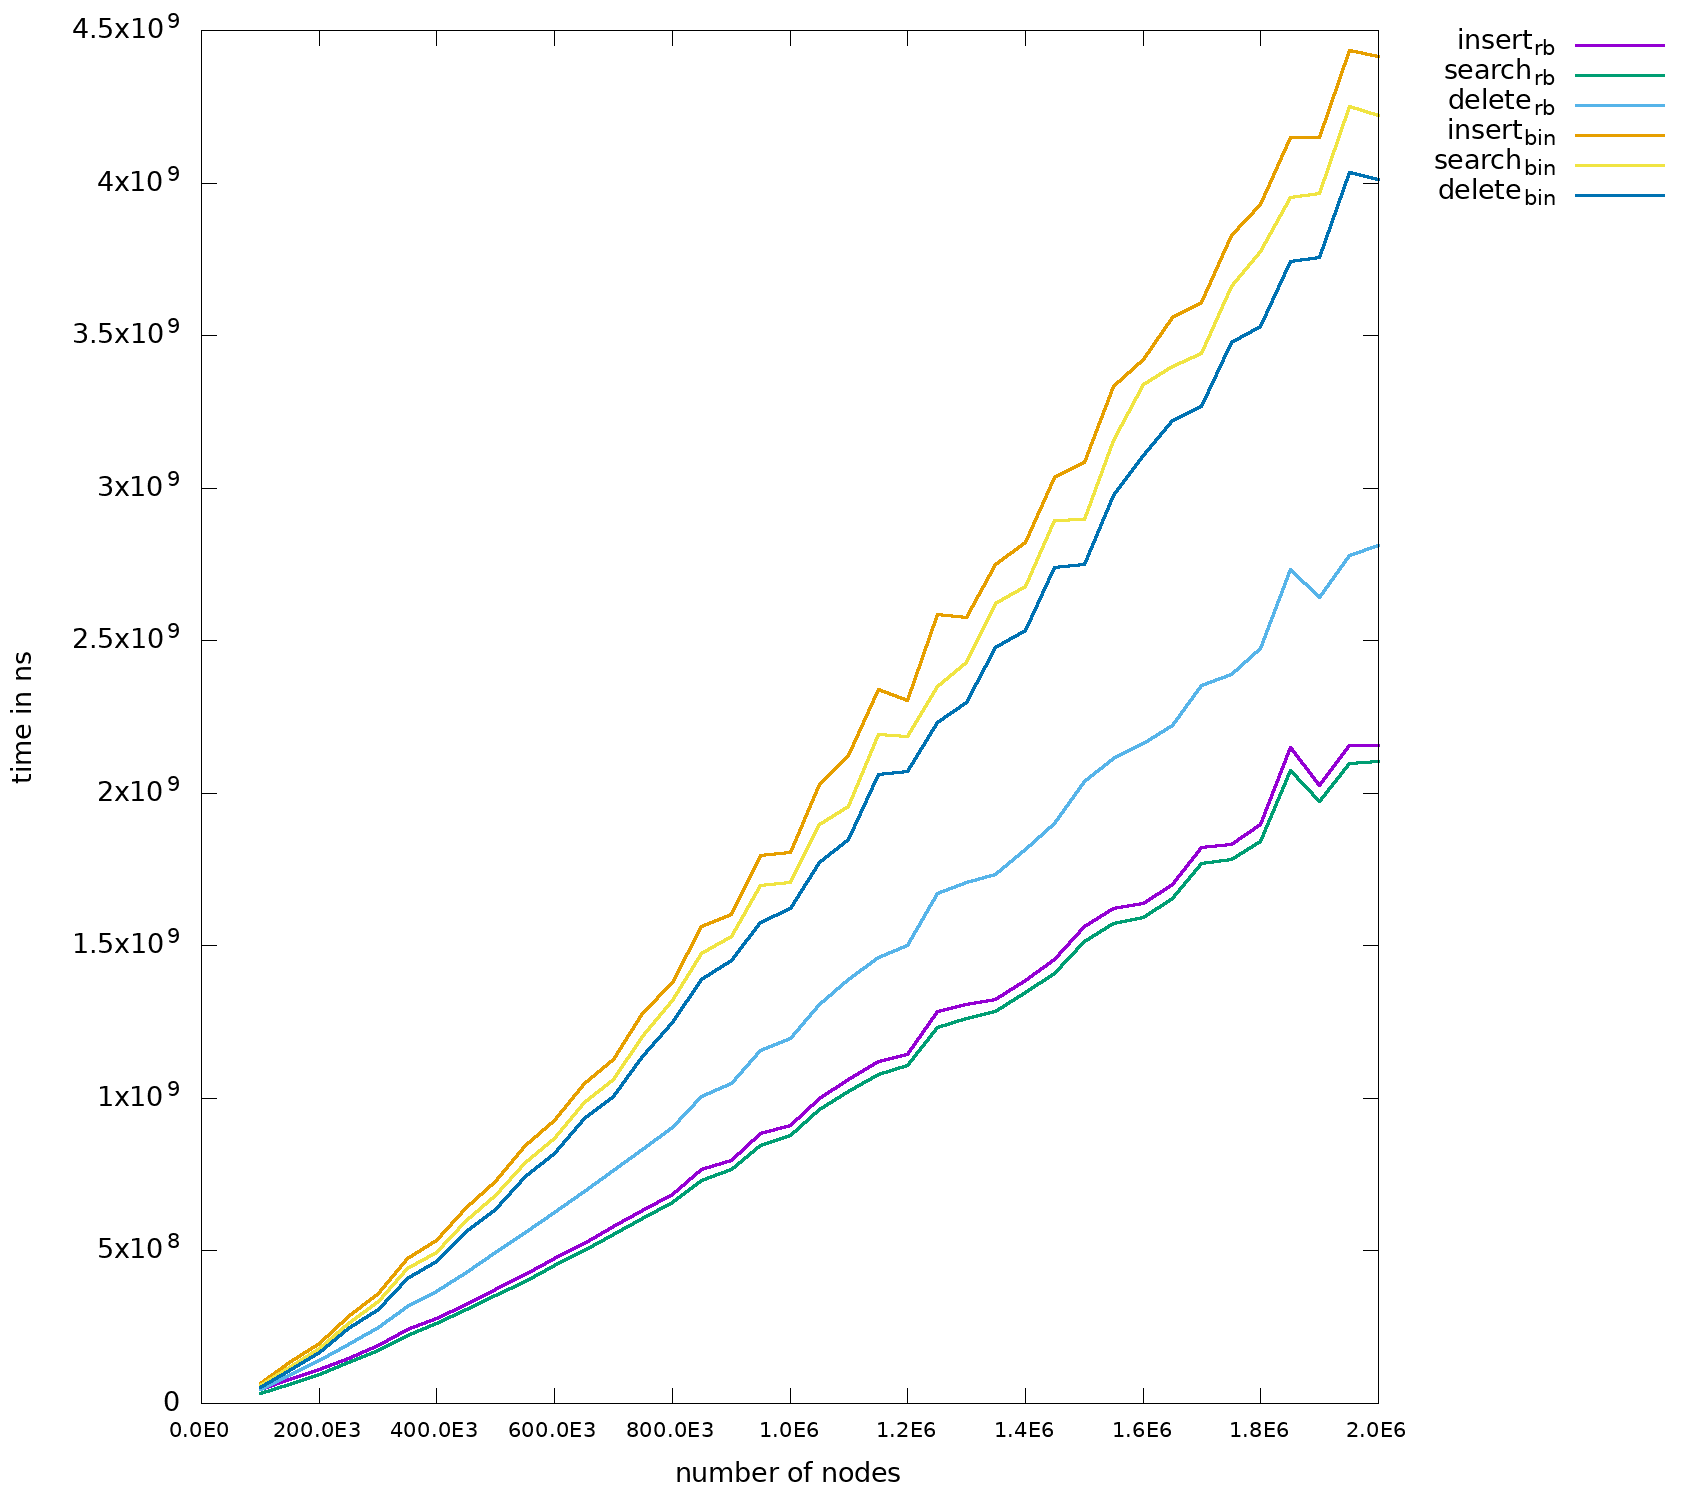
\includegraphics[width=200px]{../benchmark/compare_bin.png}
  \vspace{-20pt}
  \caption{Vergleich Laufzeit \gls{rbt}/\gls{bt}}
  \vspace{-15pt}
\end{wrapfigure}

Besonders wichtig ist es zu zeigen, dass unsere "Verbesserung" normaler Binary Trees tatsächlich performanter ist. In nebenstehender Abbildung kann man die Ergebnisse des Benchmarks erkennen.
Die Graphen, die mit dem Index $_{rb}$ beschriftet sind, sind die des \gls{rbt} und die anderen gehören zum \gls{bt}.
Man kann erkennen, dass alle Operationen beim \gls{rbt} grundsätzlich schneller als die der Standardimplementierung sind. 
Der Unterschied zwischen den beiden Datenstrukturen ist nicht konstant, sondern nimmt mit steigender Anzahl an Knoten immer weiter zu. 

Den Grund dafür kann man sehen, wenn man die Höhen der beiden Bäume vergleicht. Man kann sehen, dass sich der \gls{rbt} viel näher an der Höhe des vollständig balancierten Baumes befindet, 
als der \gls{bt}. Das sorgt dafür, dass man beim \gls{rbt} im Durchschnitt nicht so viele Vergleiche benötigt, bis man den Knoten erreicht, den man sucht oder einen \lstin{NULL}-Pointer, bei dem 
man einen neuen Knoten in den Baum einfügt. Das macht sich in den Benchmarks eindeutig bemerkbar.  

\begin{figure}[h]
  \centering
  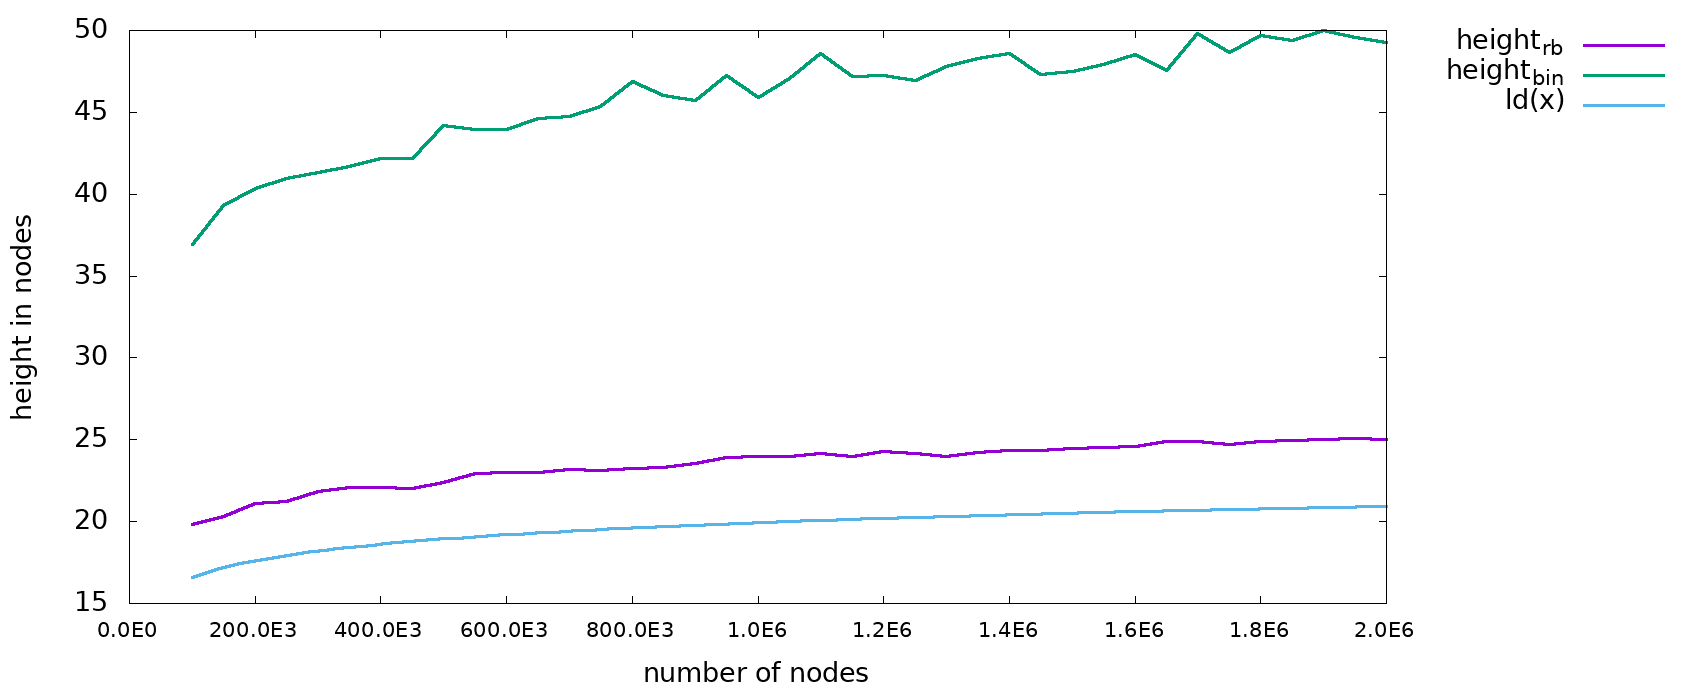
\includegraphics[width=400px]{../benchmark/compare_height.png}
  \caption{Vergleich der Höhen}
\end{figure}

Eine weitere interessante Beobachtung ist, dass die Suche und das Einfügen beim \gls{rbt} ungefähr gleich schnell sind, während das Löschen etwas langsamer als diese beiden Operationen ist.
Einen so starken Unterschied gibt es beim \gls{bt} nicht. Meine Hypothese dafür ist, dass das Rebalancieren beim Löschen von Knoten sehr viel langsamer ist, als das Rebalancieren beim Einfügen, weil
der Algorithmus häufig den ganzen Baum bis zur Root durchgeht. 

\subsection{Rekursiv vs. Iterativ} \label{ben2}

\begin{wrapfigure}{r}{200px}
  \centering
  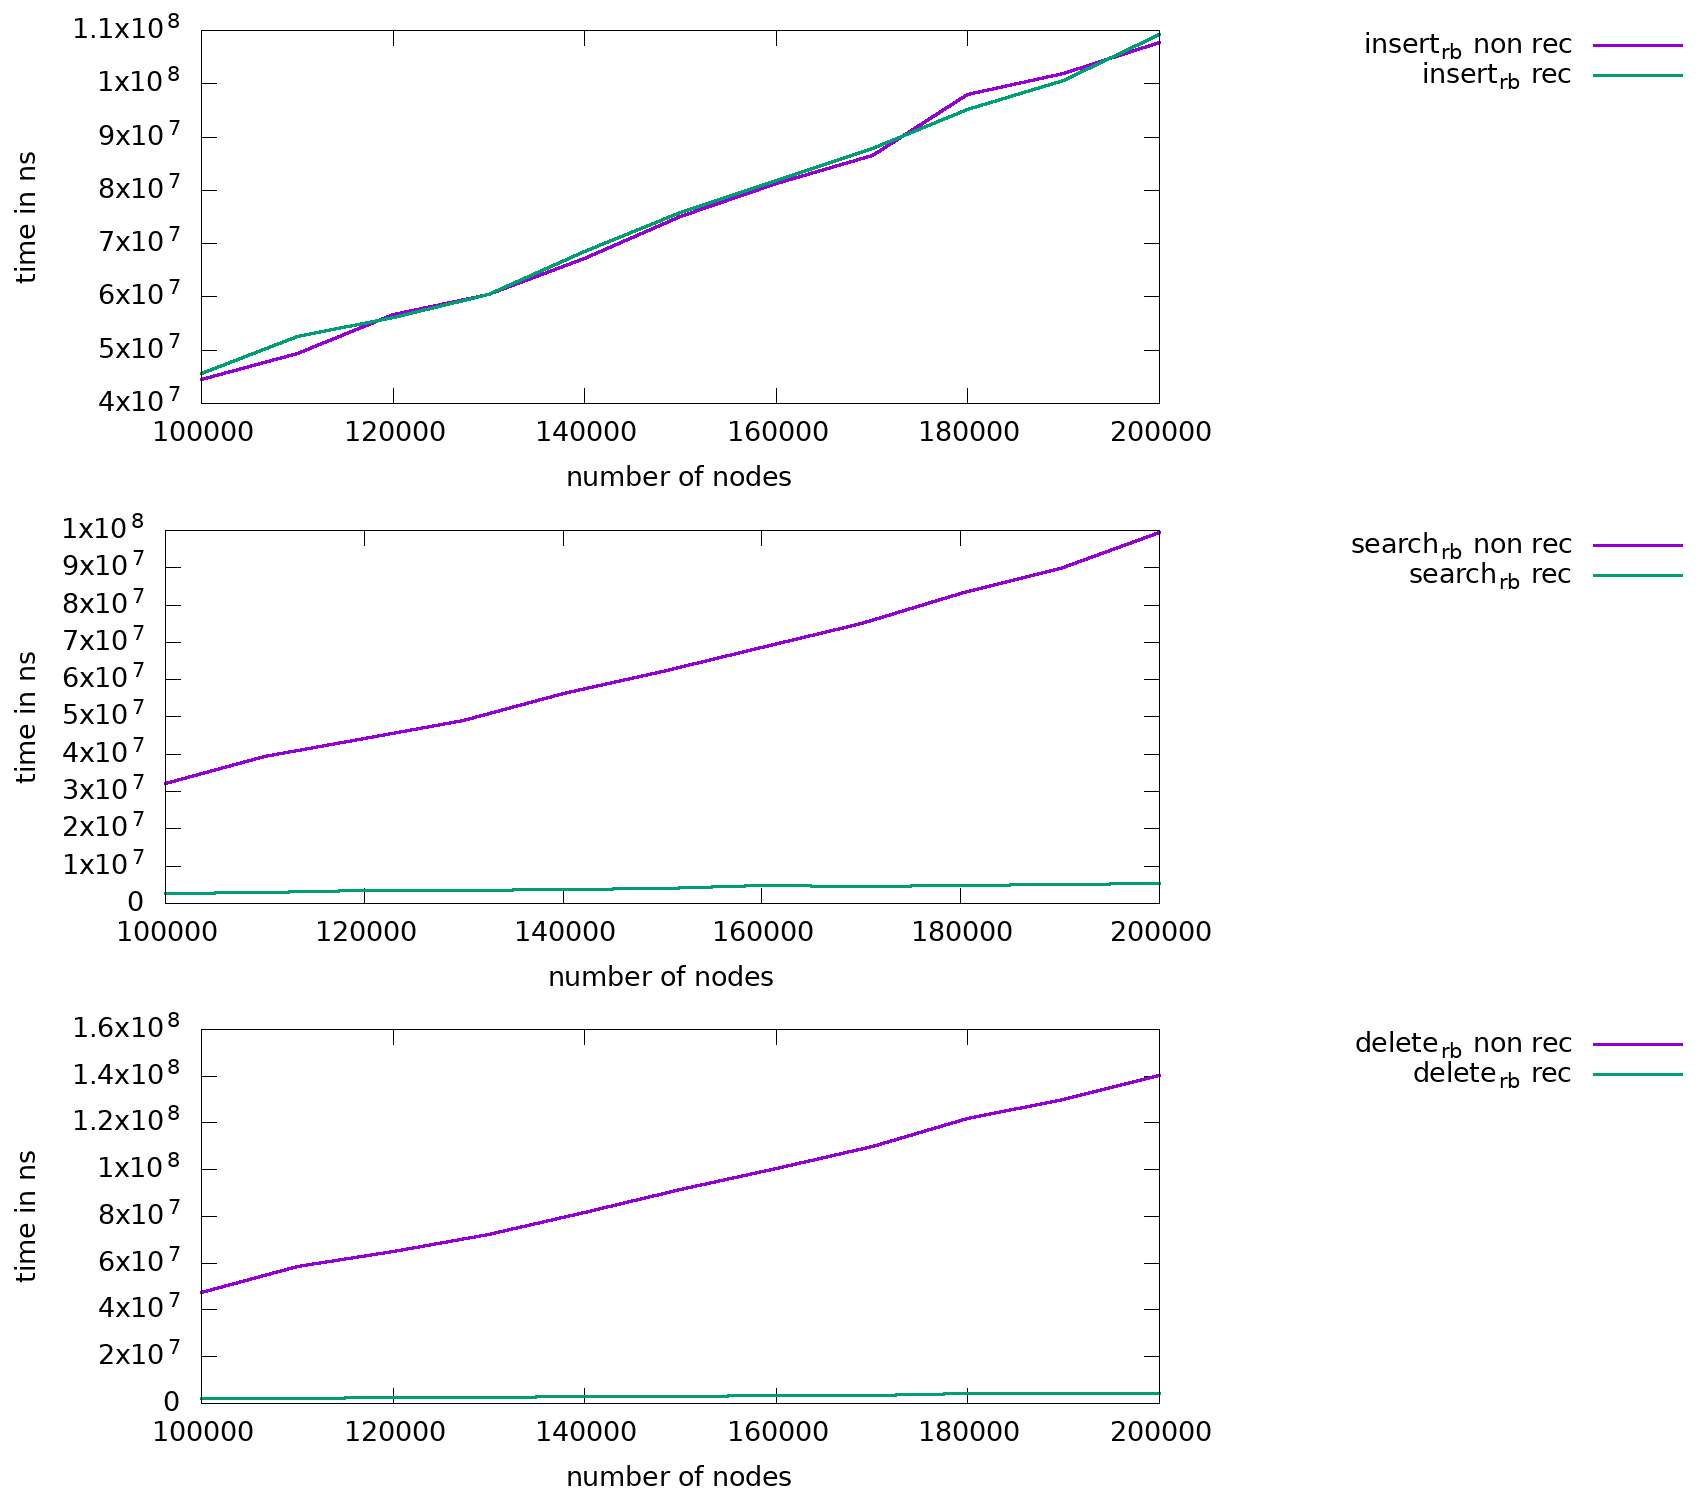
\includegraphics[width=200px]{../benchmark/compare_insert.png}
  \caption{Vergleich Rekursive/Iterative Implementierungen}
  \label{bir}
\end{wrapfigure}

Eine wichtige Frage, die sich während der Implementierung gestellt hat ist, ob man die Operationen vom \gls{rbt} iterativ oder rekursiv implementiert. 
\gls{rec} wäre zwar die erste Sache, an die man dabei denkt, weil die Definition von Bäumen auch meistens rekursiv ist. Außerdem werden auch alle Algorithmen rekursiv beschrieben. 
Das Problem daran ist, dass durch sehr große Rekursionstiefe eventuell Leistungsprobleme entstehen können und teilweise auch sehr viel Speicher nötig ist. 
Deswegen wurde, wie schon in vorhergenden Kapiteln beschrieben, eine iterative und eine rekursive Version der \gls{dt} erstellt, um diese zu vergleichen.
Das Benchmark wurde wie im vorhergehenden Abschnitt \ref{bbrbt} durchgeführt, nur wurden hier die 2 verschiedenen Versionen des Programms getestet.
Dafür wurde das Pythonscript verändert, sodass es zuerst die iterative Variante kompiliert und die Tests ausführt und in eine Datei schreibt und anschließend das selbe für die Rekursive durchführt. 

Die Ergebnisse sind in nachfolgenden Graphen in Abbildung \ref{bir} zu sehen. Es gibt jeweils einen Graph für die Suche, das Einfügen und das Löschen.

Man kann in allen drei Fällen erkennen, dass die iterative Variante (non rec) ab einer sehr großen Anzahl von Knoten konsistent schneller ist als die Rekursive (rec).
Meine Vermutung ist, dass bei Bäumen mit einer sehr großen Baumhöhe sehr viele Stackframes aufgebaut und auch wieder abgebaut werden müssen, wenn der rekursive Code ausgeführt wird.
Bei meiner anderen Implementierung gibt es einen Softwarestack, welcher nur die nötigen Daten speichert und sich auch nicht vergrößern muss, weil er schon mit der richtigen Größe erstellt wird.
Das könnte für den signifikanten Unterschied in der Laufzeit der beiden Varianten führen.

\section{Zeitkomplexität} \label{time}

Der \gls{rbt} hat im \gls{nc} die selbe Komplexität wie der \gls{bt}. Dort gibt es keine Verbesserung.
Was man jedoch sehen kann ist, dass im \gls{wcf} die Komplexität von $O(ld(n))$ erhalten bleibt, während sie beim \gls{bt} zu $O(n)$ wird.
Das liegt daran, dass die Standardimplementierung der Binary Trees keine Balancierung vornimmt. D.h., wenn man Daten in sortierter Reigenfolge einfügt, 
erhält man eine Linked List, weil immer nur einer der Unterbäume besetzt wird, je nachdem ob die Daten aufsteigend oder absteigend sortiert sind. Die Eigenschaft, 
dass man nach jedem Vergleich ca. die Hälfte der Daten nicht mehr abarbeiten muss, geht dadurch verloren. 
Nun ist es so, dass man Baumstrukturen genau zum effizienten Suchen verwenden möchte. Aus diesem Grund ist es besonders wichtig, dass man die schnelle Suche auch im Worst Case beibehält.

\begin{figure}[h]
  \centering  
  \caption{Zeit-Komplexität}
  \begin{tabular}{|c|c|c|c|} 
    \hline
    - & Suche & Einfügen & Löschen \\ 
    \hline
    Binary Tree (\gls{nc}) & $O(ld(n))$ & $O(ld(n))$ & $O(ld(n))$ \\ 
    \hline
    Binary Tree (\gls{wcf}) & $O(n)$ & $O(n)$ & $O(n)$ \\ 
    \hline
    Red Black Tree (\gls{nc}) & $O(ld(n))$ & $O(ld(n))$ & $O(ld(n))$ \\ 
    \hline
    Red Black Tree (\gls{wcf}) & $O(ld(n))$ & $O(ld(n))$ & $O(ld(n))$ \\ 
    \hline
  \end{tabular}
\end{figure}
\cite[S.215, S. 227f]{aic}

Der \gls{wcf} beim \gls{rbt} wird dann erreicht, wenn es einen alternierenden Path gibt, d.h., einen Path, in dem sich die Farben der Knoten immer abwechseln.
Dieser kann die doppelte Länge im Vergleich zu einem Path erreichen, in dem sich nur schwarze Knoten befinden.
Dieses Beispiel zeigt auch noch einmal, dass es sich bei \gls{rbt} nicht um vollständig balancierte Bäume handelt. Sie sind lediglich balancierte Bäume, die den \gls{wcf}, zu einer linearen Datenstruktur zu werden, vermeiden.
In der unteren Abbildung sind die Knoten, in denen eine dick gedruckte Linie \textbf{endet} jeweils rot und alle anderen schwarz.  

\begin{figure}[h]
  \centering
  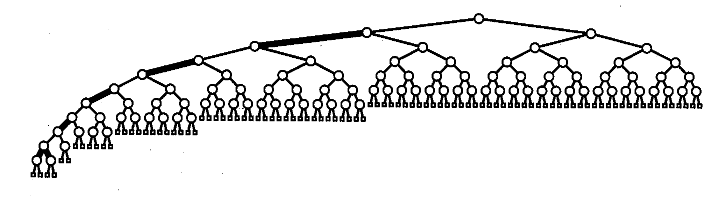
\includegraphics[width=400px]{worst_case.png}
  \caption{Worst Case \gls{rbt}: Path mit alternierender Farbe}
\end{figure}
\cite[S. 228]{aic}

\pagebreak
\section{Fazit}

In der Arbeit wurden die beiden Datenstrukturen \gls{rbt} und \gls{bt} erst theoretisch definiert 
und dann eine praktische Implementierung des \gls{rbt} erfolgreich umgesetzt. Es wurde ebenfalls ein \gls{bt} implementiert, 
worauf aber nicht direkt eingegangen wurde. Seine Implementierung wurde lediglich für das Benchmarking benötigt.
Es wurden außerdem verschiedene Ansätze aufgezeigt, wie man einen \gls{rbt} direkt umsetzten kann, und klar gemacht, warum welcher Ansatz gewählt wurde und welche Vor- und Nachteile das mit sich bringt.

Durch ausführliches Benchmarking konnte aufgezeigt werden, dass der \gls{rbt} tatsächlich eine bessere Performance in Bezug auf die Laufzeit aufweist.
Das wurde nochmal theoretisch mit der Diskussion der Zeitkomplexität untermauert. 

Dem Leser wurde ein umfangreicher Überblick über das Thema geboten und Möglichkeiten, dieses weiter zu erkunden, 
indem er die noch offenen Fragen selbst versucht, zu beantworten. 

\pagebreak
\begingroup
\parindent 0pt
\parskip 2ex
\def\enotesize{\normalsize}
\theendnotes
\endgroup

\pagebreak
\vspace*{\fill}
\begin{center}
  
\includegraphics[width=400px]{selbst.png}  
\end{center}
\vspace*{\fill}

\pagebreak
\bibliographystyle{alpha}
\bibliography{references} % see references.bib for bibliography management

\end{document}
